% ******************************* PhD Thesis Template **************************
% Please have a look at the README.md file for info on how to use the template

\documentclass[oneside,a4paper,13pt,bookman,numbered,print,index]{Classes/CSEThesisPSnPDF}
%\usepackage[utf8]{inputenc} % This for vietnamese 
%\usepackage[utf8]{vietnam} % This for vietnamese 

% ******************************************************************************
% ******************************* Class Options ********************************
% *********************** See README for more details **************************
% ******************************************************************************

% `a4paper'(The University of Cambridge PhD thesis guidelines recommends a page
% size a4 - default option) or `a5paper': A5 Paper size is also allowed as per
% the Cambridge University Engineering Deparment guidelines for PhD thesis
%
% `11pt' or `12pt'(default): Font Size 10pt is NOT recommended by the University
% guidelines
%
% `oneside' or `twoside'(default): Printing double side (twoside) or single
% side.
%
% `print': Use `print' for print version with appropriate margins and page
% layout. Leaving the options field blank will activate Online version.
%
% `index': For index at the end of the thesis
%
% `draftclassic': For draft mode without loading any images (same as draft in book)
%
% `draft': Special draft mode with line numbers, images, and water mark with
% timestamp and custom text. Position of the text can also be modified.
%
% `abstract': To generate only the title page and abstract page with
% dissertation title and name, to submit to the Student Registry
%
% `chapter`: This option enables only the specified chapter and it's references
%  Useful for review and corrections.
%
% ************************* Custom Page Margins ********************************
%
% `custommargin`: Use `custommargin' in options to activate custom page margins,
% which can be defined in the preamble.tex. Custom margin will override
% print/online margin setup.
%
% *********************** Choosing the Fonts in Class Options ******************
%
% `times' : Times font with math support. (The Cambridge University guidelines
% recommend using times)
%
% `fourier': Utopia Font with Fourier Math font (Font has to be installed)
%            It's a free font.
%
% `customfont': Use `customfont' option in the document class and load the
% package in the preamble.tex
%
% default or leave empty: `Latin Modern' font will be loaded.
%
% ********************** Choosing the Bibliography style ***********************
%
% `authoryear': For author-year citation eg., Krishna (2013)
%
% `numbered': (Default Option) For numbered and sorted citation e.g., [1,5,2]
%
% `custombib': Define your own bibliography style in the `preamble.tex' file.
%              `\RequirePackage[square, sort, numbers, authoryear]{natbib}'.
%              This can be also used to load biblatex instead of natbib
%              (See Preamble)
%
% **************************** Choosing the Page Style *************************
%
% `default (leave empty)': For Page Numbers in Header (Left Even, Right Odd) and
% Chapter Name in Header (Right Even) and Section Name (Left Odd). Blank Footer.
%
% `PageStyleI': Chapter Name next & Page Number on Even Side (Left Even).
% Section Name & Page Number in Header on Odd Side (Right Odd). Footer is empty.
%
% `PageStyleII': Chapter Name on Even Side (Left Even) in Header. Section Number
% and Section Name in Header on Odd Side (Right Odd). Page numbering in footer


% ********************************** Preamble **********************************
% Preamble: Contains packages and user-defined commands and settings
% ******************************************************************************
% ****************************** Custom Margin *********************************

% Add `custommargin' in the document class options to use this section
% Set {innerside margin / outerside margin / topmargin / bottom margin}  and
% other page dimensions
\ifsetCustomMargin
  \RequirePackage[left=30mm,right=30mm,top=35mm,bottom=30mm]{geometry}
  \setFancyHdr % To apply fancy header after geometry package is loaded
\fi

% Add spaces between paragraphs
%\setlength{\parskip}{0.5em}
% Ragged bottom avoids extra whitespaces between paragraphs
\raggedbottom
% To remove the excess top spacing for enumeration, list and description
%\usepackage{enumitem}
%\setlist[enumerate,itemize,description]{topsep=0em}

% *****************************************************************************
% ******************* Fonts (like different typewriter fonts etc.)*************

% Add `customfont' in the document class option to use this section

\ifsetCustomFont
  % Set your custom font here and use `customfont' in options. Leave empty to
  % load computer modern font (default LaTeX font).
  %\RequirePackage{helvet}

  % For use with XeLaTeX
  %  \setmainfont[
  %    Path              = ./libertine/opentype/,
  %    Extension         = .otf,
  %    UprightFont = LinLibertine_R,
  %    BoldFont = LinLibertine_RZ, % Linux Libertine O Regular Semibold
  %    ItalicFont = LinLibertine_RI,
  %    BoldItalicFont = LinLibertine_RZI, % Linux Libertine O Regular Semibold Italic
  %  ]
  %  {libertine}
  %  % load font from system font
  %  \newfontfamily\libertinesystemfont{Linux Libertine O}
\fi

% *****************************************************************************
% **************************** Custom Packages ********************************

% ************************* Algorithms and Pseudocode **************************

%\usepackage{algpseudocode}


% ********************Captions and Hyperreferencing / URL **********************

% Captions: This makes captions of figures use a boldfaced small font.
%\RequirePackage[small,bf]{caption}

\RequirePackage[labelsep=space,tableposition=top]{caption}
\renewcommand{\figurename}{Fig.} %to support older versions of captions.sty


% *************************** Graphics and figures *****************************

%\usepackage{rotating}
%\usepackage{wrapfig}

% Uncomment the following two lines to force Latex to place the figure.
% Use [H] when including graphics. Note 'H' instead of 'h'
\usepackage{float}
%\restylefloat{figure}

% Subcaption package is also available in the sty folder you can use that by
% uncommenting the following line
% This is for people stuck with older versions of texlive
%\usepackage{sty/caption/subcaption}
\usepackage{subcaption}

% ********************************** Tables ************************************
\usepackage{booktabs} % For professional looking tables
\usepackage{multirow}

%\usepackage{multicol}
%\usepackage{longtable}
%\usepackage{tabularx}


% *********************************** SI Units *********************************
\usepackage{siunitx} % use this package module for SI units


% ******************************* Line Spacing *********************************

% Choose linespacing as appropriate. Default is one-half line spacing as per the
% University guidelines

%\doublespacing
%\onehalfspacing
%\singlespacing


% ************************ Formatting / Footnote *******************************

% Don't break enumeration (etc.) across pages in an ugly manner (default 10000)
%\clubpenalty=500
%\widowpenalty=500

%\usepackage[perpage]{footmisc} %Range of footnote options


% *****************************************************************************
% *************************** Bibliography  and References ********************

%\usepackage{cleveref} %Referencing without need to explicitly state fig /table

% Add `custombib' in the document class option to use this section
\ifuseCustomBib
   \RequirePackage[square, sort, numbers, authoryear]{natbib} % CustomBib

% If you would like to use biblatex for your reference management, as opposed to the default `natbibpackage` pass the option `custombib` in the document class. Comment out the previous line to make sure you don't load the natbib package. Uncomment the following lines and specify the location of references.bib file

%\RequirePackage[backend=biber, style=numeric-comp, citestyle=numeric, sorting=nty, natbib=true]{biblatex}
%\bibliography{References/references} %Location of references.bib only for biblatex

\fi

% changes the default name `Bibliography` -> `References'
\renewcommand{\bibname}{References}


% ******************************************************************************
% ************************* User Defined Commands ******************************
% ******************************************************************************

% *********** To change the name of Table of Contents / LOF and LOT ************

%\renewcommand{\contentsname}{My Table of Contents}
%\renewcommand{\listfigurename}{My List of Figures}
%\renewcommand{\listtablename}{My List of Tables}


% ********************** TOC depth and numbering depth *************************

\setcounter{secnumdepth}{3}
\setcounter{tocdepth}{2}


% ******************************* Nomenclature *********************************

% To change the name of the Nomenclature section, uncomment the following line

%\renewcommand{\nomname}{Symbols}


% ********************************* Appendix ***********************************

% The default value of both \appendixtocname and \appendixpagename is `Appendices'. These names can all be changed via:

%\renewcommand{\appendixtocname}{List of appendices}
%\renewcommand{\appendixname}{Appndx}
%\renewcommand{\appendixtocname}{List of appendices}
%\renewcommand{\appendixname}{Phụ lục}


% *********************** Configure Draft Mode **********************************

% Uncomment to disable figures in `draft'
%\setkeys{Gin}{draft=true}  % set draft to false to enable figures in `draft'

% These options are active only during the draft mode
% Default text is "Draft"
%\SetDraftText{DRAFT}

% Default Watermark location is top. Location (top/bottom)
%\SetDraftWMPosition{bottom}

% Draft Version - default is v1.0
%\SetDraftVersion{v1.1}

% Draft Text grayscale value (should be between 0-black and 1-white)
% Default value is 0.75
%\SetDraftGrayScale{0.8}


% ******************************** Todo Notes **********************************
%% Uncomment the following lines to have todonotes.

%\ifsetDraft
%	\usepackage[colorinlistoftodos]{todonotes}
%	\newcommand{\mynote}[1]{\todo[author=kks32,size=\small,inline,color=green!40]{#1}}
%\else
%	\newcommand{\mynote}[1]{}
%	\newcommand{\listoftodos}{}
%\fi

% Example todo: \mynote{Hey! I have a note}


% ************************ Thesis Information & Meta-data **********************
% Thesis title and author information, refernce file for biblatex
% ************************ Thesis Information & Meta-data **********************
%% The title of the thesis
\singlespacing \title{Thiết kế sản phẩm móc khóa thông minh (Smart Keyring) dựa trên nền tảng công nghệ Bluetooth Low Energy (BLE)}
%\texorpdfstring is used for PDF metadata. Usage:
%\texorpdfstring{LaTeX_Version}{PDF Version (non-latex)} eg.,
%\texorpdfstring{$sigma$}{sigma}

%% Subtitle (Optional)
%\part{title}\subtitle{Using the CUED template}

%% University and Crest
%\university{HO CHI MINH CITY UNIVERSITY OF TECHNOLOGY}
\university{ĐẠI HỌC QUỐC GIA THÀNH PHỐ CHÍ MINH\\TRƯỜNG ĐẠI HỌC BÁCH KHOA}
%% Department (eg. Department of Engineering, Maths, Physics)
%\dept{FACULTY OF COMPUTER SCIENCE AND ENGINEERING}
\dept{KHOA KHOA HỌC VÀ KỸ THUẬT MÁY TÍNH}

% Crest minimum should be 30mm.
\crest{
\includegraphics[width=0.2\textwidth]{bklogo}}
%% Use this crest, if you are using the college crest

%% Crest long miminum should be 65mm
%\crest{\inc\dfrac{lu}{den}degraphics[width=0.45\textwidth]{University_Crest_Long}}

%% College shield [optional]
% Crest minimum should be 30mm.
%\collegeshield{
\includegraphics[width=0.2\textwidth]{CollegeShields/Kings}}


%% Supervisor (optional)
%% for multiple supervisors, append each supervisor with the \newline command
\supervisor{\textbf{TS. Phạm Hoàng Anh}}
%\newline
%Prof. C.D. Supervisor\newline
%Prof. E.F. Supervisor\newline
%Prof. G.H. Supervisor}}

%% Supervisor Role (optional) - Supervisor (default) or advisor
%\supervisorrole{\textbf{Giảng viên hướng dẫn}}
\supervisorrole{{Giảng viên hướng dẫn:}}
%% if no title is desired:
% \supervisorrole{}

%% Advisor (optional)
%% for multiple advisors, append each advisor with the \newline command
%\advisor{Advisor 1\newline
%Advisors 2\newline
%Advisor 3\newline
%Advisor 4}

%% Advisor Role (optional) - Advisor (default) or leave empty
% \advisorrole{Advisors: }
%% if no title is required
% \advisorrole{}

%% The full name of the author
\author{51203774 - Trương Hoài Thương\newline
	51204417 - Võ Tấn Tùng}
\authorrole{Sinh viên thực hiện:}

%% You can redefine the submission text:
% Default as per the University guidelines:
% ``This dissertation is submitted for the degree of''
%\renewcommand{\submissiontext}{change the default text here if needed}

%% Full title of the Degree
\degreetitle{Thuộc chương trình hỗ trợ sinh viên kỹ sư tài năng tham gia NCKH}

%% College affiliation (optional)
%\college{King's College}

%% Submission date
% Default is set as {\monthname[\the\month]\space\the\year}
\degreedate{Tháng 11 Năm 2016}

%% Meta information
\subject{LaTeX} \keywords{{LaTeX} {Thesis} {Computer Engineering}}


% ***************************** Abstract Separate ******************************
% To printout only the titlepage and the abstract with the PhD title and the
% author name for submission to the Student Registry, use the `abstract' option in
% the document class.

%\ifdefineAbstract
% \pagestyle{empty}
% \includeonly{Declaration/declaration, Abstract/abstract}
%\fi

% ***************************** Chapter Mode ***********************************
% The chapter mode allows user to only print particular chapters with references
% Title, Contents, Frontmatter are disabled by default
% Useful option to review a particular chapter or to send it to supervisior.
% To use choose `chapter' option in the document class

%\ifdefineChapter
% \includeonly{Chapter3/chapter3}
%\fi

% ******************************** Front Matter ********************************
\begin{document}

\frontmatter
\maketitle

\doublespacing
% ******************************* Thesis Declaration ***************************

\begin{declaration}

Nhóm chúng tôi cam đoan ngoài những nguồn trích dẫn tham khảo được nhắc đến chi tiết trong bài viết, những nội dung còn lại trong bài là bản gốc và chưa được đăng và xem xét ở bất kỳ trung tâm nghiên cứu cũng như trường đại học nào khác. Bài nghiên cứu khoa học này là thành quả của chính chúng tôi và không bao gồm thành quả của các nghiên cứu khác ngoại trừ những giúp đỡ trong mục lời cảm ơn.

\end{declaration}


% ************************** Thesis Acknowledgements **************************

\begin{acknowledgements}
\title{Lời Cảm ơn}      


Nhóm chúng tôi muốn gửi lời cảm ơn tới Trường Đại học Bách khoa TP.HCM đã tài trợ đề tài, tạo điều kiện hiện thực đề tài và lời cảm ơn giáo viên hướng dẫn TS. Phạm Hoàng Anh đã hướng dẫn định hướng phát triển đề tài cũng như tài trợ thiết bị nghiên cứu.

\end{acknowledgements}

% ************************** Thesis Abstract *****************************
% Use `abstract' as an option in the document class to print only the titlepage and the abstract.
\begin{abstract}
\renewcommand{\abstractname}{Tóm Tắt}

Trong bản thuyết trình này, nhóm chúng tôi sẽ giới thiệu về công nghệ Bluetooth Low Energy (BLE) và khả năng ứng dụng thực tiễn và hiện thực thiết kế sản phẩm móc khóa thông minh dựa trên nền tảng công nghệ BLE và lập trình ứng dụng di động sử dụng công nghệ này.

Tài liệu sẽ gồm có 3 phần chính: 

• Tổng quan: giới thiệu về công nghệ BLE, các thiết bị phần cứng đang được phát triển và ứng dụng. 

• Thiết kế và hiện thực sản phẩm móc khóa: xác định mục tiêu ứng dụng và lựa chọn thiết bị phần cứng, thiết kế mô hình thiết bị và giao thức với ứng dụng thiết bị di động, lập trình ứng dụng dành co hệ điều hành Android.

• Thử nghiệm và kết quả đạt được: thử nghiệm khả năng ứng dụng thiết bị trong thực tế.

• Tổng kết: rút ra các kết luận nhận xét về kết quả đạt được và hướng phát triển trong tương lai.

\end{abstract}


% *********************** Adding TOC and List of Figures ***********************
\onehalfspacing
\tableofcontents
\listoffigures
\listoftables

% \printnomenclature[space] space can be set as 2em between symbol and description
%\printnomenclature[3em]
\doublespacing
\printnomenclature

% ******************************** Main Matter *********************************
\mainmatter

%*******************************************************************************
%*********************************** First Chapter *****************************
%*******************************************************************************

\chapter{Tổng quan}  %Title of the First Chapter

\ifpdf
    \graphicspath{{Chapter1/Figs/Raster/}{Chapter1/Figs/PDF/}{Chapter1/Figs/}{}}
\else
    \graphicspath{{Chapter1/Figs/Vector/}{Chapter1/Figs/}}
\fi


%********************************** %First Section  **************************************
\section{Mở đầu} %Section - 1.1 
\subsection{Mục đích đề tài và tính cấp bách}
Trong cuộc sống bận rộn hiện nay, con người chúng ta hay có xu hướng bị xao nhãng và bỏ quên các thiết bị nhỏ. trong đó có thiết bị điện thoại di động và chùm chìa khóa là hai vật rất quan trọng và thường hay bỏ quên nhất. Và tìm kiếm chúng không hề dễ dàng, nhất là khi đang vội thì sẽ làm mọi thứ rối tung lên.

Và đồng thời hiện nay công nghệ phát triển cho các thiết bị kết nối không dây phát triển mạnh, có thể ứng dụng cho nhiều lĩnh vực. Bluetooth Low Energy là một trong những cái tên nổi bật nhất trong các công nghệ truyền dữ liệu không dây bởi đặc tính tiện lợi, phổ biến và tiết kiệm năng lượng. Và nhóm chúng tôi muốn tìm hiểu và ứng dụng công nghệ này vào cuộc sống thực tiễn.

Từ điều đó đã thúc đẩy nhóm chúng tôi tìm cách giải quyết và nảy ra ý tưởng tạo ra sản phẩm móc khóa thông mình - Smart Keyring có chức năng kết nối với thiết bị di động sử dụng công nghệ BLE để giải quyết vấn đề trên dựa trên các tính năng của BLE.
\subsection{Mô tả đề tài}

Đề tài sẽ chia làm 2 phần chính:

• \textbf{Sản phẩm móc khóa}: 1 thiết bị có kích thước nhỏ, năng lượng tiêu thụ ít. 

Chức năng:

- Báo hiệu bằng âm thanh và ánh sáng khi có yêu cầu định vị.

- Điều khiển chức năng định vị trên thiết bị di động qua nút ấn.
	
- Báo hiệu khi mất kết nối với thiết bị di động.
		

• \textbf{Ứng dụng di động}: ứng dụng chạy trên nền tảng Android. 

Chức năng:

- Gửi yêu cầu định vị tới sản phẩm móc khóa để kích hoạt tính năng báo hiệu trên móc khóa.

- Báo hiệu bằng âm thanh yêu cầu định vị.

- Báo hiệu khi bị mất kết nối với sản phẩm móc khóa.

\subsection{Mục tiêu - Phạm vi - Đối tượng nghiên cứu}

Xuất phát từ các lý do trình bày ở trên, chúng tôi đã thực hiện đề tài “Thiết kế sản phẩm móc khóa thông minh (Smart Keyring) dựa trên nền tảng công nghệ Bluetooth Low Energy (BLE)”. Mục tiêu của đề tài là:

• Tìm hiểu về công nghệ Bluetooth Low Energy

• Kế thiết bị “Móc khóa thông minh - SmartKeyring” sử dụng công nghệ

Bluetooth và kết nối với ứng dụng Android trên điện thoại.

\nomenclature[z-cif]{$CIF$}{Cauchy's Integral Formula}                                % first letter Z is for Acronyms 
\nomenclature[a-F]{$F$}{complex function}                                                   % first letter A is for Roman symbols
\nomenclature[g-p]{$\pi$}{ $\simeq 3.14\ldots$}                                             % first letter G is for Greek Symbols
\nomenclature[g-i]{$\iota$}{unit imaginary number $\sqrt{-1}$}                      % first letter G is for Greek Symbols
\nomenclature[g-g]{$\gamma$}{a simply closed curve on a complex plane}  % first letter G is for Greek Symbols
\nomenclature[x-i]{$\oint_\gamma$}{integration around a curve $\gamma$} % first letter X is for Other Symbols
\nomenclature[r-j]{$j$}{superscript index}                                                       % first letter R is for superscripts
\nomenclature[s-0]{$0$}{subscript index}                                                        % first letter S is for subscripts

%TODO: BLE bỏ ở đây có hợp lý không?
%********************************** % Third Section  *************************************
\section{Bluetooth Low Energy (BLE) }  %Section - 1.3 
\label{section1.3} %TODO ref htelectronic
Như đã được đề cập ở mục \ref{history}, BLE xuất hiện từ phiên bản 4.0, là một bước ngoặc lớn trong sự phát triển kết nối không dây. Các mạch BLE rất nhỏ cùng với công suất tiêu thụ hiệu năng cực thấp (khoảng vài chục uA khi hoạt động), nên hầu hết các thiết bị đều có thể tích hợp công nghệ này, từ các thiết bị nhỏ bé như tai nghe, chìa khóa.. cho tới các thiết bị lớn như tủ lạnh, tivi, xe máy... Nhờ đó, các thiết bị có thể trở nên "smart".

\subsection{Khái niệm và lịch sử phát triển Bluetooth}
Bluetooth là công nghệ không dây cho phép các thiết bị điện, điện tử giao tiếp với nhau trong khoảng cách ngắn, bằng sóng vô tuyến qua băng tần chung ISM (Industrial, Scientific, Medical) trong dãy tầng 2.40- 2.48 GHz. Đây là dãy băng tầng không cần đăng ký được dành riêng để dùng cho các thiết bị không dây trong công nghiệp, khoa học, y tế.

	\begin{table}[ht]
		\begin{tabular}{ |c|m{2cm}|m{2cm}|m{2cm}|m{2cm}| } 
			\hline
			& \textbf{Bluetooth} & \textbf{BLE} & \textbf{Wifi} & \textbf{Zigbee} \\ 
			\hline
			\textbf{Radio Frequency} &	2.4G &	2.4G &	2.4G &	2.4G \\ 
			\hline
			\textbf{Distance Range} &	10m	&>60m &	30m	& 10-100m \\ 
			\hline
			\textbf{Air Datarate} &	1-3Mbps &	1Mbps &	54Mbps &	250kbps \\
			\hline
			\textbf{Application Throughput} &	0.7-2.1Mbps &	305kbps &Depend &120kbps\\
			\hline
			\textbf{Security} &	64bit, 128bit &	128-bit & AES	SSID, WEP&	128-bit AES \\
			\hline
			\textbf{Power consumption}&	Low	&Very Low&	High&	Low \\
			\hline
			\textbf{Certification Body}&	Bluetooth SIG&	Bluetooth SIG&	IEEE802.11&	IEEE802.15.4 \\
			\hline
			\textbf{Network topology} &	Point-to-Point Scatternet&	Point-to-Point Star&	Point-to-Hub& 		Mesh, Ad-hoc\\
			\hline
		\end{tabular}
		\caption {Bảng so sánh các công nghệ truyền không dây}
		\label{table:1.1}
	\end{table}

\begin{figure}[ht]
	\centering    
	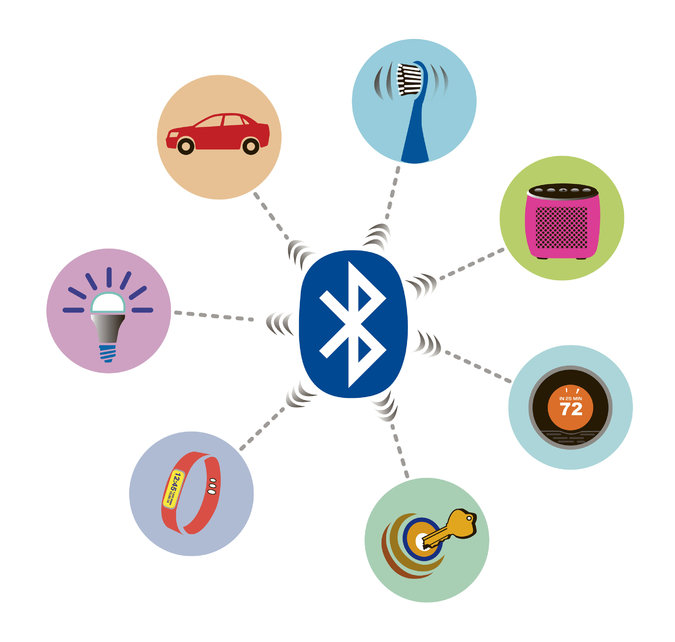
\includegraphics[width=0.7\textwidth]{btuse}
	\caption[Các ứng dụng Bluetooth]{Các ứng dụng Bluetooth}
	\label{fig:btuse}
\end{figure}

Lịch sử phát triển:

•Bluetooth 4.0 - Bluetooth Low Energy: Là sự kết hợp của các đời Bluetooth trước đó với nhau. Bluetooth 4.0 đạt tốc độ truyền tải lên đến 25Mbps, dễ dàng ghép đôi các thiết bị với nhau, hiệu năng tiêu thụ thấp. Đây là chuẩn Bluetooth được sử dụng trên hầu hết các thiết bị hiện nay.

•Bluetooth 4.1 và 4.2: Là phiên bản ra đời đầu năm 2014 với nhiều cải tiến vượt bậc so với Bluetooth 4.0 như khả năng điều chống chồng chéo tín hiệu, kết nối thực sự thông minh và khả năng truyền dữ liệu độc lập mà không cần phụ thuôc vào trung tâm điều khiển. Phiên bản 4.2 được phát triển có khả năng truyền tải cao và bảo mật hơn, nhưng quan trọng hơn cả là cho phép các vi xử lý sử dụng chuẩn giao thức Ipv6 để truy cập trực tiếp vào internet.

•Bluetooth 5.0: theo dự kiến sẽ bắt đầu xuất hiện trên các thiết bị thương mại vào cuối 2016 nay hoặc đầu năm 2017 (Q1). Bluetooth 5.0 có tầm phủ sóng tăng lên gấp 4 lần so với Bluetooth 4.2 hiện nay, còn tốc độ truyền dữ liệu thì tăng lên cao nhất là 2 lần. Việc mở rộng khả năng phủ sóng của Bluetooth sẽ giúp các thiết bị Internet of Things sẽ có thể giao tiếp với nhau cũng như với trạm điều khiển một cách dễ dàng hơn, vượt qua bức tường của một căn nhà bình thường, trong khi lại tăng tốc thu thập và truyền dữ liệu. Chuẩn Bluetooth mới cũng sẽ giúp các beacon và giải pháp nhận diện địa điểm trở nên thông minh, chính xác và phản hồi nhanh hơn với sự hiện diện của người dùng.

\subsection{Phân loại vai trò thiết bị BLE}
Có 4 loại thiết bị BLE (có thể gọi là chế độ hoạt động) đó là Peripheral, Central, Observer và Broadcaster và bình thường thì một thiết bị BLE chỉ hoạt động  trong một chế độ.

• \textbf{Central} là thiết bị sẽ chủ động yêu cầu kết nối đến các thiết bị BLE khác (thường là smartphone, tablet). Sau khi kết nối thì chúng ta lại gọi BLE Central là  BLE Master.

• \textbf{BLE Peripheral} là thiết bị chấp nhận yêu cầu kết nối (thường là đồ vật BLE). Tương tự, sau khi kết nối thì chúng ta gọi BLE Peripheral là BLE Slave.

• \textbf{BLE Observer} là BLE Central nhưng chỉ nhận dữ liệu nhận dạng của các thiết bị xung quanh nhưng không bao giờ tạo kết nối

• \textbf{BLE Broadcaster} là BLE Peripheral chỉ phát dữ liệu nhận dạng nhưng không bao giờ chấp nhận yêu cầu kết nối từ các BLE Central.
\newpage

\subsection{Cách thức hoạt động của BLE}
%TODO HTeletronic
Theo chuẩn BLE định nghĩa thì các thiết bị BLE có 4 hoạt động cơ bản như sau:

• \textbf{Advertising}: là hoạt động phát dữ liệu nhận dạng cơ bản của thiết bị BLE Peripheral ra môi trường xung quanh trước khi kết nối

• \textbf{Scanning}: là hoạt động của thiết bị BLE Central để thu thập dữ liệu nhận dạng của nhiều thiết bị BLE Peripheral xung quanh

• \textbf{Connecting}: là hoạt động của cả thiết bị BLE Central và BLE peripheral trong đó thiết bị BLE Central có thể gửi yêu cầu thêm thông tin nhận dạng (gọi là Scan Request) và BLE Peripheral gửi theo yêu cầu (gọi là Scan Response). Sau đó BLE Central sẽ kiểm tra đầy đủ thông tin nhận dạng (từ Advertising data và từ Scan Response data) và gửi yêu cầu kết nối (gọi là Connection Request), cuối cùng thiết bị BLE Peripheral sẽ trả lời chấp nhận hay từ chối kết nối (gọi là Connection Response)

• \textbf{Discovering}: là hoạt động của thiết bị BLE Client sau khi kết nối nhằm lấy thông tin về các loại dữ liệu mà thiết bị BLE Server có thể cung cấp. Ví dụ, thiết bị BLE Server có thể có dữ liệu về gia tốc, hoặc có dữ liệu về nhiệt độ, độ ẩm, v.v.. và thiết bị BLE Client sẽ có nhu cầu biết các loại dữ liệu nào có thể nhận từ BLE Server

Cách thức hoạt động của BLE ở hình \ref{fig: btwork}:
	\begin{figure}[h]
		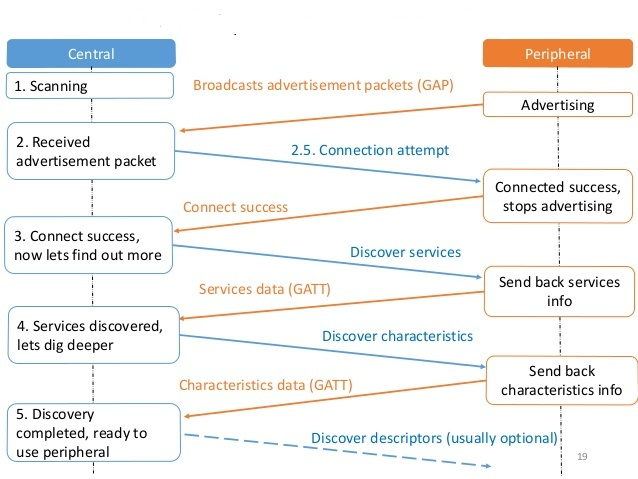
\includegraphics[width=1.0\textwidth]{btwork}
		\caption[Sơ đồ hoạt động của BLE]{Sơ đồ hoạt động của BLE}
		\label{fig: btwork}
	\end{figure}
	
\newpage
\subsection{Các vi điều khiển tích hợp công nghệ BLE}
%TODO : ref http://www.argenox.com/bluetooth-low-energy-ble-v4-0-development/library/a-guide-to-selecting-a-bluetooth-chipset/
Các SoC tích hợp sẵn công nghệ BLE phố biến có thể kể đến:

• Texas Instruments: CC2540/CC2541, dòng CC256x, CC26xx

• Nordic Semiconductor: nRF51822, nRF8001

• CSR CSR101x

• Cypress Semiconductor PSoC 4 BLE / PRoC BLE

Tuy nhiên ở Việt Nam tại thời điểm bắt đầu nghiên cứu và hiện thực đề tài thì 2 loại chipset phổ biến và có giá tiền phổ thông là CC2540 và CC2541 được cung cấp theo dạng Module HM-10.
	\begin{figure}[h]
		\centering    
		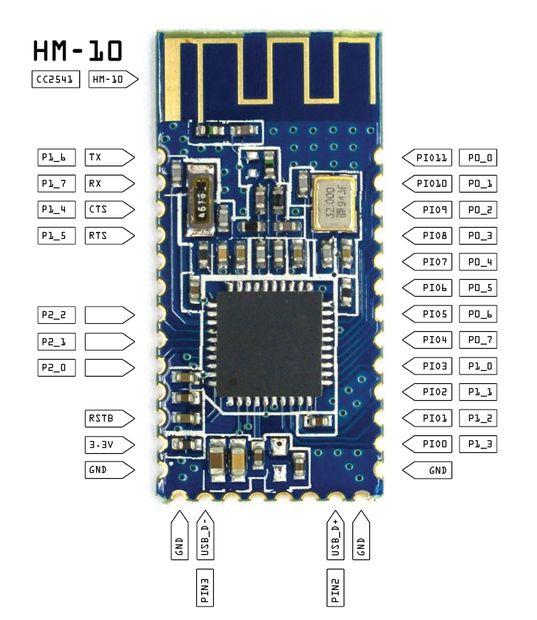
\includegraphics[width=0.4\textwidth]{hm10}
		\caption[Module HM-10]{Module HM-10}
		\label{fig: hm10}
	\end{figure}

\nomenclature[z-FEM]{FEM}{Finite Element Method}
\nomenclature[z-PFEM]{PFEM}{Particle Finite Element Method}
\nomenclature[z-FVM]{FVM}{Finite Volume Method}
\nomenclature[z-BEM]{BEM}{Boundary Element Method}
\nomenclature[z-MPM]{MPM}{Material Point Method}
\nomenclature[z-LBM]{LBM}{Lattice Boltzmann Method}
\nomenclature[z-MRT]{MRT}{Multi-Relaxation 
Time}
\nomenclature[z-RVE]{RVE}{Representative Elemental Volume}
\nomenclature[z-GPU]{GPU}{Graphics Processing Unit}
\nomenclature[z-SH]{SH}{Savage Hutter}
\nomenclature[z-CFD]{CFD}{Computational Fluid Dynamics}
\nomenclature[z-LES]{LES}{Large Eddy Simulation}
\nomenclature[z-FLOP]{FLOP}{Floating Point Operations}
\nomenclature[z-ALU]{ALU}{Arithmetic Logic Unit}
\nomenclature[z-FPU]{FPU}{Floating Point Unit}
\nomenclature[z-SM]{SM}{Streaming Multiprocessors}
\nomenclature[z-PCI]{PCI}{Peripheral Component Interconnect}
\nomenclature[z-CK]{CK}{Carman - Kozeny}
\nomenclature[z-CD]{CD}{Contact Dynamics}
\nomenclature[z-DNS]{DNS}{Direct Numerical Simulation}
\nomenclature[z-EFG]{EFG}{Element-Free Galerkin}
\nomenclature[z-PIC]{PIC}{Particle-in-cell}
\nomenclature[z-USF]{USF}{Update Stress First}
\nomenclature[z-USL]{USL}{Update Stress Last}
\nomenclature[s-crit]{crit}{Critical state}
\nomenclature[z-DKT]{DKT}{Draft Kiss Tumble}
\nomenclature[z-PPC]{PPC}{Particles per cell}
%*******************************************************************************
%****************************** Second Chapter *********************************
%*******************************************************************************

\chapter{Thiết kế và hiện thực \newline sản phẩm móc khóa thông minh - Smart Keyring}

\ifpdf
    \graphicspath{{Chapter2/Figs/Raster/}{Chapter2/Figs/PDF/}{Chapter2/Figs/}}
\else
    \graphicspath{{Chapter2/Figs/Vector/}{Chapter2/Figs/}}
\fi


%\section[Short title]{Reasonably long section title}
\section{Thiết kế tính năng sản phẩm}
% Uncomment this line, when you have siunitx package loaded.
%The SI Units for dynamic viscosity is \si{\newton\second\per\metre\squared}.
\textit{Thiết kế tính năng sản phẩm:}

\label{feature}
Sản phẩm Smart Keyring sẽ có các tính năng cơ bản như:

• Báo hiệu khi mất kết nối: hỗ trợ việc cảnh báo người tránh bỏ quên 1 trong 2 thiết bị.

• Báo hiệu khi kích hoạt chức năng tìm kiếm: cho phép người dùng định vị thiết bị còn lại trong phạm vi kết nối.

• Hai chế độ báo hiệu bằng âm thanh hoặc ánh sáng đèn led hoặc cả 2: mục đích sử dụng trong nhiều trường hợp khác nhau như đêm tối, không gian yên tĩnh...
\section{Các hướng tiếp cận vấn đề}

Tại thời điểm tìm hiểu và hiện thực đề tài NCKH, tại Việt Nam chỉ có module HM-10 có sử dụng chip BLE CC2540/2541 được phát triển thành board mạch hoàn chỉnh nên phần này chỉ nói về hướng phát triển với board mạch này.

\subsection{Phát triển thiết bị chỉ dựa vào SoC CC2540/2541}
\label{dev}
Về hướng này chúng ta sẽ phát triển lập trình thiết bị chỉ trên duy nhất 1 SoC CC2540/2541.

\textbf{Ưu điểm}: 

• Có thể thu nhỏ thiết kế đến mức tối thiểu

• Viết ứng dụng ngay trên nền tảng BLE sẽ tiết kiệm tối đa năng lượng tiêu thụ.

\textbf{Nhược điểm}: 

• Bị hạn chế về khả năng phát triển cả về phần cứng lẫn phần mềm.

• Không tìm được source code firmware cho module.

• Không có tài liệu chính thống nào hướng dẫn các bước lập trình cho vi điều khiển CC2540/2541 được tích hợp trên module HM-10

• Nhà sản xuất không công khai thiết kế mạch của sản phẩm HM-10

• Chỉ có duy nhất 1 phần mềm hỗ trợ các gói thư viện lập trình cho CC2540/2541 là IAR Embedded Workbench for 8051 \cite{iar} hỗ trợ Texas Instrument nhưng bản quyền cho phần mềm có giá quá cao và các thư viện này sử dụng mã nguồn đóng nên không chuyển sang các phần mềm khác được.

\textit{Vì những cản trở đó, nhóm quyết định chuyển sang phương pháp tiếp cận khác đơn giản và khả thi hơn.}

\subsection{Kết hợp MCU và Module BLE HM-10}
Cách tiếp cận này khá quen thuộc với đa số hệ thống và sản phẩm hiện nay bao gồm 1 vi điều khiển trung tâm: chứa toàn bộ chương trình hoạt động của sản phẩm và các thiết bị ngoại vi (sensor, các module giao tiếp rf, Bluetooth…)

\textbf{Ưu điểm: }

• Dễ tiếp cận, do người hiện thực có thể kiểm soát được công nghệ mình sử dụng

• Tùy biến các loại vi điều khiển sao cho thích hợp nhất đối với yêu cầu đề tài. Các vi điều khiển riêng rẻ hiện nay rất đa dạng chủng loại và chức năng, đi kèm theo nó là hệ thống hỗ trợ cực kì tốt từ nhà sản xuất về tài liệu, môi trường lập trình, các forum trao đổi. điển hình là các thương hiệu Atmel, Microchip…

\textbf{Nhược điểm:} 

• Đối nghịch lại với ưu điểm của cách tiếp cận đầu tiên thì hướng tiếp cận này sẽ cần nhiều không gian hơn (thêm 1 vi điều khiển).

• Làm cho hệ thống mất đi tính linh động và gọn nhẹ so với tính chất sản phẩm cũng như là năng lượng tiêu thụ không được tối ưu.

• Thêm 1 vi điều khiển tương đương với việc thêm 1 nguồn tiêu thụ điện, giảm thời gian hoạt động của sản phẩm.

\section{Sơ đồ hoạt động}
\subsection{Tổng quát}
Sơ đồ hoạt động tổng quát:

\begin{figure}[h]
	\centering    
	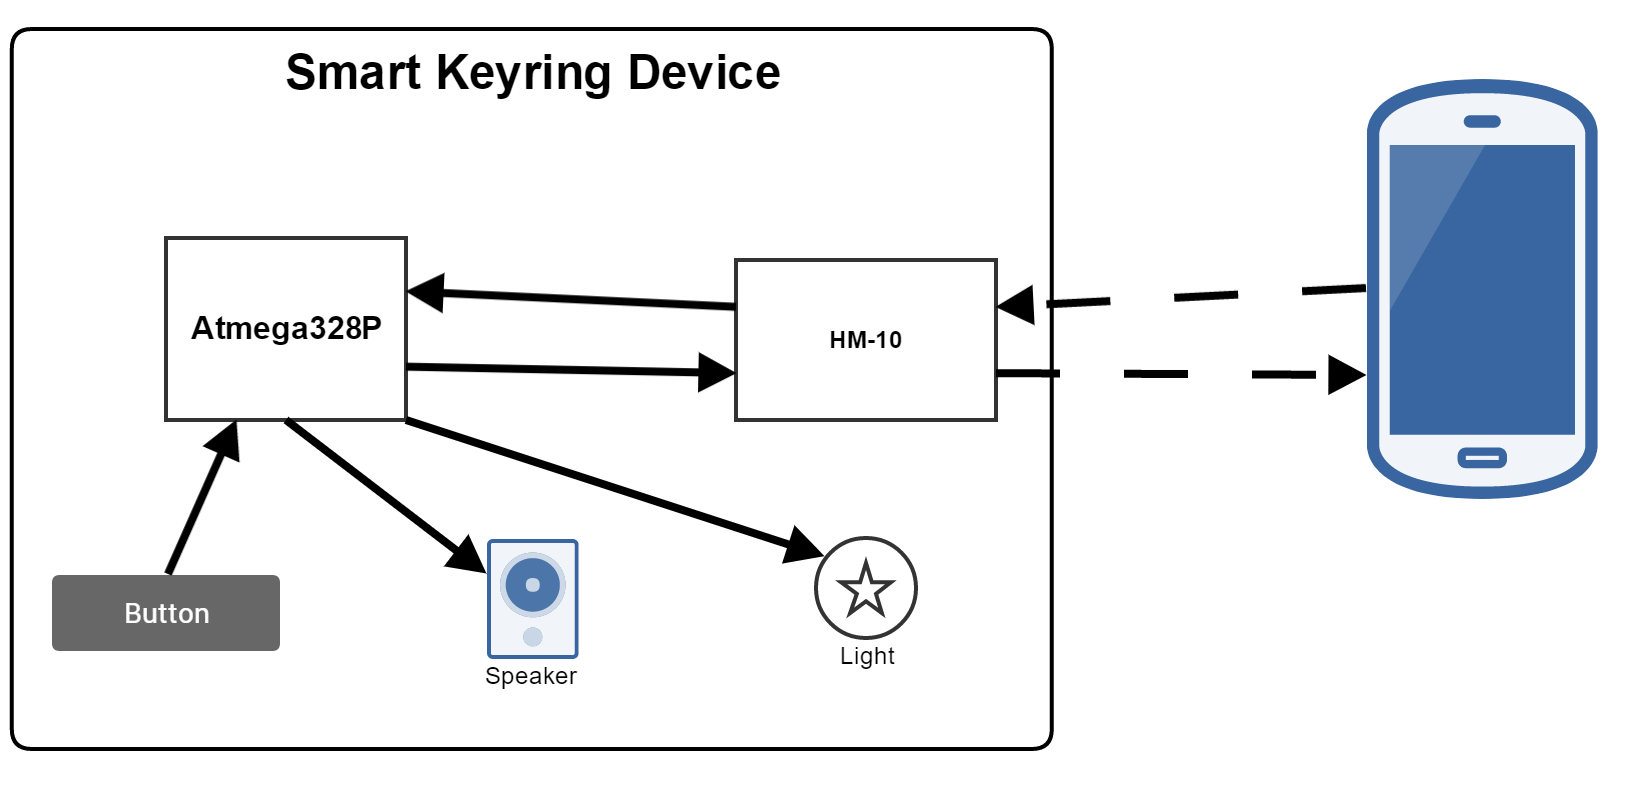
\includegraphics[width=1.0\textwidth]{general}
	\caption[Sơ đồ hoạt động tổng quát]{Sơ đồ hoạt động tổng quát}
	\label{fig: general}
\end{figure}

Như hình \ref{fig: general}, thiết bị Smart Keyring giao tiếp với thiết bị di động thông qua module BLE HM-10 và được điều khiển bởi MCU ATmega328P đảm nhận chức năng quản lý I/O như nút ấn, loa báo hiệu và đèn cũng như là truyền nhận thông điệp với module HM10.

\subsection{Nhận lệnh báo từ thiết bị di động}

Chức năng tìm kiếm thiết bị được kích hoạt bởi thiết bị di động được mô tả ở hình \ref{fig: ring1}.

Trình tự các hoạt động như sau:

(1) Thiết bị di động gửi gói tin với nội dung yêu cầu phát tín hiệu báo tới module HM-10.

(2) MCU ATmega328P nhận gói tin từ module HM-10 bằng giao thức UART với chế độ interrupt.

(3) Loa và đèn báo hiệu được kích hoạt tùy theo nội dung gói tin: kích hoạt cả hai hoặc chỉ kích hoạt đèn báo hiệu

(4*) Nút nhấn có chức năng ngắt chế độ báo hiệu khi cần thiết thông qua interrupt GPIO

\begin{figure}[h]
	\centering    
	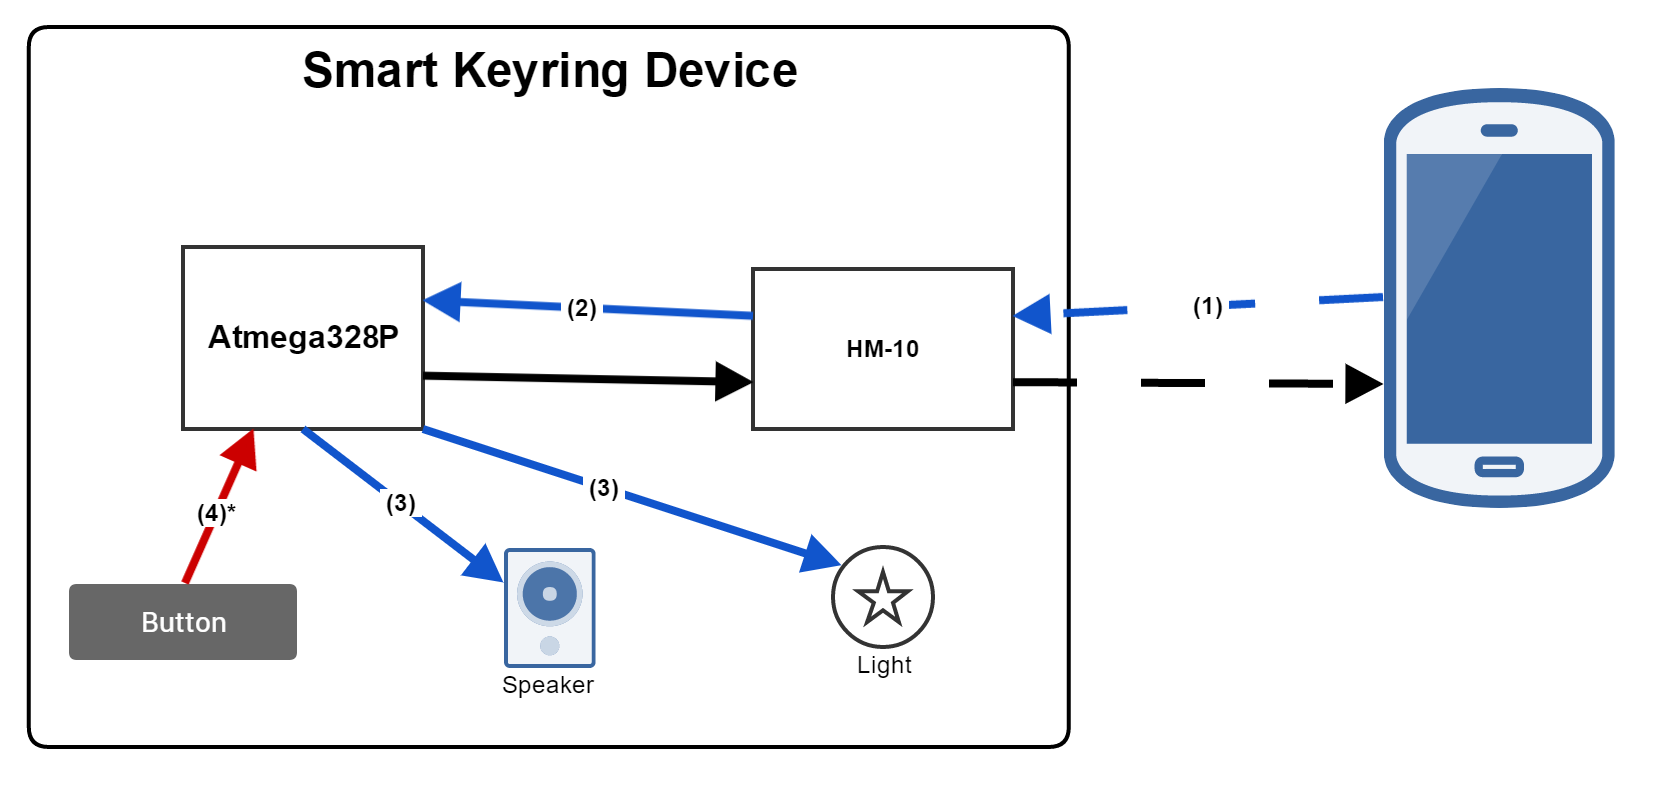
\includegraphics[width=1.0\textwidth]{ring1}
	\caption[Sơ đồ hoạt động khi nhận lệnh báo từ thiết bị di động]{Sơ đồ hoạt động khi nhận lệnh báo từ thiết bị di động}
	\label{fig: ring1}
\end{figure}

Sơ đồ hoạt động trên đúng với chức năng ngắt báo hiệu thiết bị được điều khiển bởi thiết bị di động, chỉ khác tại bước (3) là ngắt loa và đèn và không có bước (4).
\subsection{Kích hoạt thiết bị di động bật chế độ báo hiệu}

Chức năng kích hoạt thiết bị di động bật chế độ báo hiệu được mô tả ở hình \ref{fig: ring2}.

Trình từ các hoạt động như sau:

(1) MCU ATmega328P nhận tín hiệu điều khiển từ nút ấn thông qua interrupt GPIO

(2) Module BLE HM-10 nhận gói tin điều khiển từ MCU ATmega328 thông qua UART

(3) Thiết bị di động nhận gói tin truyền từ Module HM-10 và kích hoạt chế độ báo hiệu

\begin{figure}[h]
	\centering    
	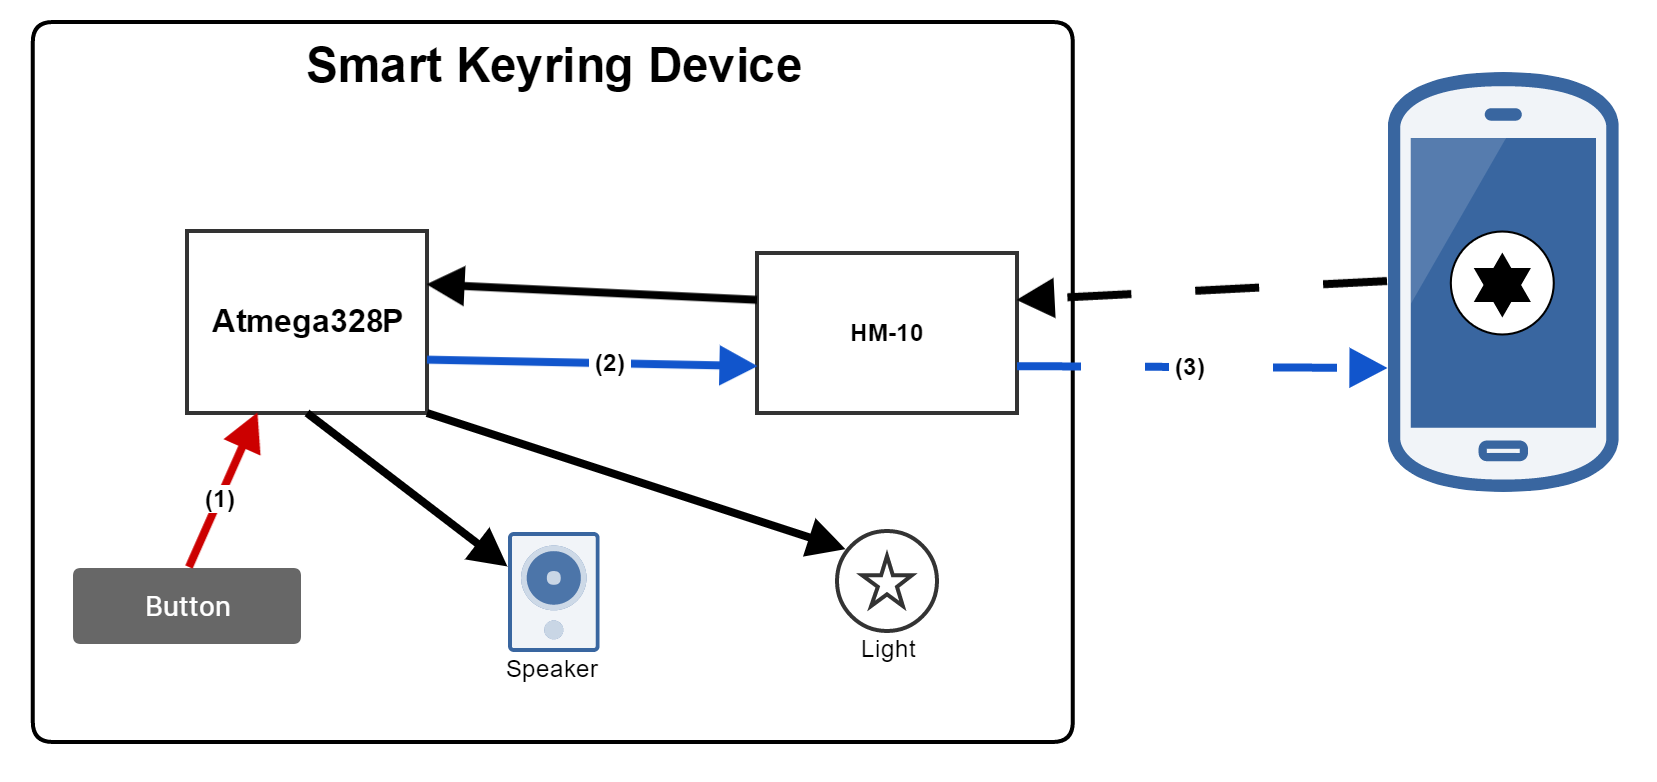
\includegraphics[width=1.0\textwidth]{ring2}
	\caption[Sơ đồ kích hoạt thiết bị di động bật chế độ báo hiệu]{Sơ đồ kích hoạt thiết bị di động bật chế độ báo hiệu}
	\label{fig: ring2}
\end{figure}
\newpage

\subsection{Sơ đồ trạng thái hoạt động khi ngắt kết nối}
%TODO: xem lại phần này
Dựa theo tính năng sản phẩm ở mục \ref{feature}, sơ đồ trạng thái hoạt động được thiết kế ở hình \ref{fig: ble} và \ref{fig: blelost}

	\begin{figure}[H]
		\centering    
		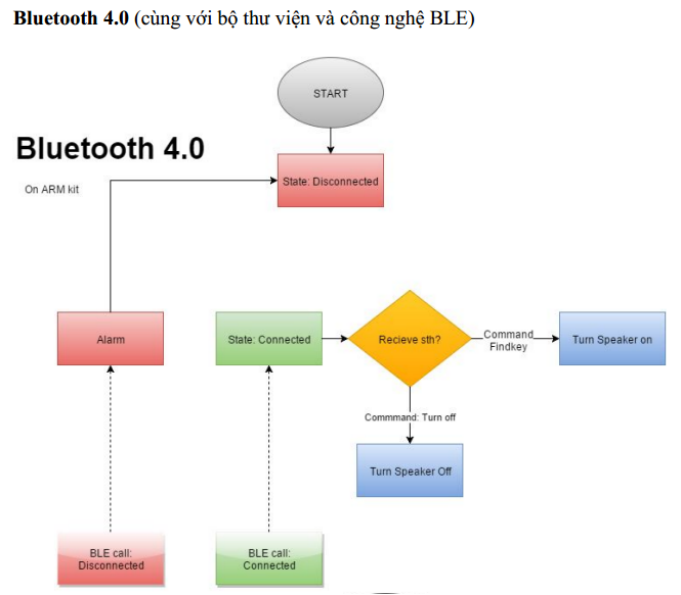
\includegraphics[width=1.0\textwidth]{ble}
		\caption[Sơ đồ trạng thái trên thiết bị Smart Keyring]{Sơ đồ trạng thái trên thiết bị Smart Keyring}
		\label{fig: ble}
	\end{figure}
	
	\begin{figure}[H]
		\centering    
		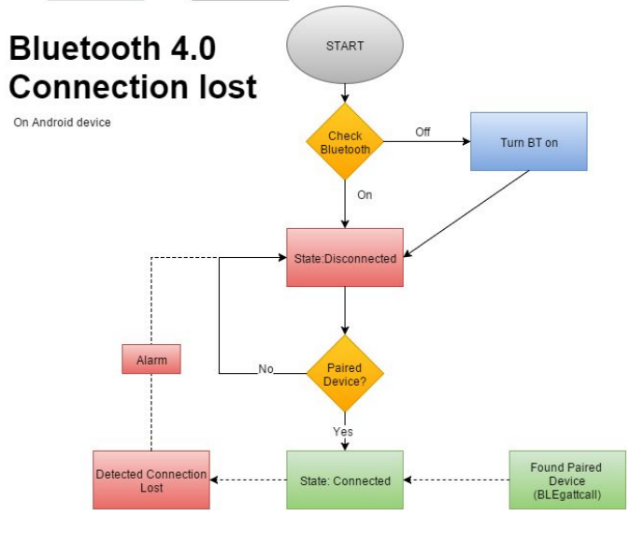
\includegraphics[width=1.0\textwidth]{blelost}
		\caption[Sơ đồ hoạt động trên thiết bị di động]{Sơ đồ hoạt động trên thiết bị di động}
		\label{fig: blelost}
	\end{figure}

\section{Hiện thực phần cứng}
\subsection{Lựa chọn linh kiện và thiết bị phần cứng}

\textit{Sản phẩm hiện thực gồm 3 phần:}

\textbf{Module giao tiếp không dây:}

Tất nhiên yêu cầu tiên quyết của sản phẩm là việc giao tiếp không dây giữa các thiết bị, tiếp theo là việc làm sao để tiết kiệm năng lượng trên từng phần của sản phẩm. Thông qua tìm hiểu, nhóm đã phát hiện ra công nghệ truyền dữ liệu không dây trong khoảng cách ngắn phổ biển nhất hiện nay là công nghệ Bluetooth Low Energy. 

Hiện nay, trên thị trường có rất nhiều loại mẫu mã và thiết kế cho module Bluetooth Low Energy từ nhiều hãng sản xuất khác nhau. Thời gian đầu lúc tiếp cận, nhóm đã lựa chọn mẫu phổ biến nhất trên thị trường hiện nay với giá thành tương đối hợp lí. Đó là module Bluetooth BLE HM-10 của hãng JNHuamao Technology Company có xuất xứ từ Trung Quốc. Sau thời gian thử nghiệm và nghiên cứu với nhiều phiên bản của sản phẩm, nhóm nhận thấy module hoạt động tốt và ổn định, thông số kỹ thuật mà nhà sản xuất cung cấp gần đúng với các thông số kỹ thuật mà nhóm rút ra được trong quá trình thử nghiệm.

\begin{figure}[h]
	\centering    
	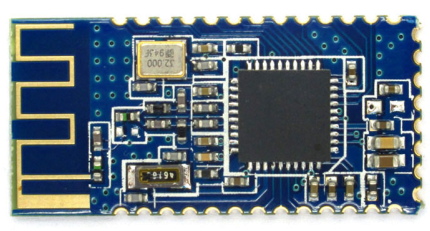
\includegraphics[width=1.0\textwidth]{hm10}
	\caption[Module BLE HM-10]{Module BLE HM-10}
	\label{fig: c2-hm10}
\end{figure}

Thông số kỹ thuật của module: (do nhà sx cung cấp)

• SoC: CC2540/2541 (tùy theo đợt sản xuất)

• BT version: Bluetooth Specification V4.0 BLE.

• Tần số hoạt động: 2.4GHz ISM band.

• RF power: -23dbm, -6dbm, 0dbm, 6dbm.

• Baudrate: hỗ trợ đến 230400, mặc định là 9600.

• Nguồn: +2.5 - 3.3VDC 50mA.

• Dòng tiêu thụ: Active mode 8.5mA, Sleep mod 50-200 uA.

• Thực nghiệm cho thấy module có thể thực hiện truyền nhận trong khoảng cách 20m – 30m( tùy vào thiết bị di động).

\textbf{Vi điều khiện trung tâm:}

Vi điều khiển trung tâm cũng cần thỏa mản một số yêu cầu sau:

• Điện áp hoạt động: 3.3V hoặc ít hơn.

• Có ít nhất 1 kênh giao tiếp UART.

• Tiết kiệm năng lượng nhiều nhất có thể.

• Công cụ lập trình dễ tiếp cận và có bộ thư viện hỗ trợ tương đối đầy đủ.

Với những yêu cầu trên, qua quá trình tìm hiểu và đúc kết kinh nghiệm từ trước, nhóm đã chọn được vi điều khiển thích hợp cho mô hình. Đó là vi điều khiển ATmega328P của hãng Atmel.

\begin{figure}[H]
	\centering    
	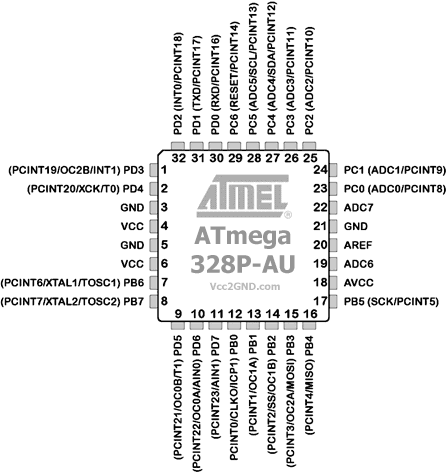
\includegraphics[width=1.0\textwidth]{atmega}
	\caption[MCU ATmega328P]{MCU ATmega328P}
	\label{fig: atmega}
\end{figure}

\textbf{Các thông số kỹ thuật:}

Core:	 AVR 8-bit

Kích thước bộ nhớ FLASH:	 32 KB Flash

Tần số hoạt động tối đa:	 20 MHz

Các chuẩn giao tiếp:	 I²C, SPI, UART/USART

Số lượng cổng GPIO:	 23

Điện áp hoạt động:	 1.8V to 5.5V

\textbf{Các thiết bị xuất nhập:}

• LED nguồn: chức năng báo hiệu khi thiết bị đang hoạt động.

• LED báo hiệu: chức năng bật tắt bằng ánh sáng LED khi có yêu cầu từ thiết bị di động.

• Buzzer: chức năng phát âm thanh khi có yêu cầu từ thiết bị di động.

• Nút bấm: chức năng kích hoạt thiết bị Smart Keyring gửi lệnh cho thiết bị di động báo chuông.

Theo như yêu cầu chức năng ở mục \ref{feature}, schematic được thiết kế như hình \ref{fig: schematic}

	\begin{figure}[H]
		\centering    
		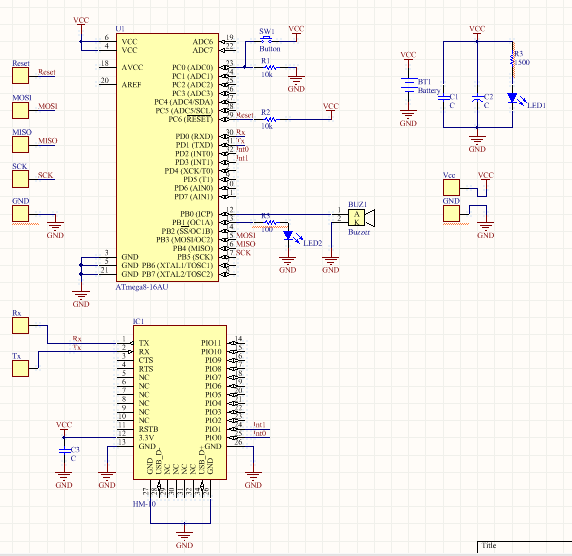
\includegraphics[width=1.0\textwidth]{schematic}
		\caption[Schematic của thiết bị Smart Keyring]{Schematic của thiết bị Smart Keyring}
		\label{fig: schematic}
	\end{figure}
	
Mạch thiết bị thử nghiệm theo schematic như hình \ref{fig: keydraft}

	\begin{figure}[H]
		\centering    
		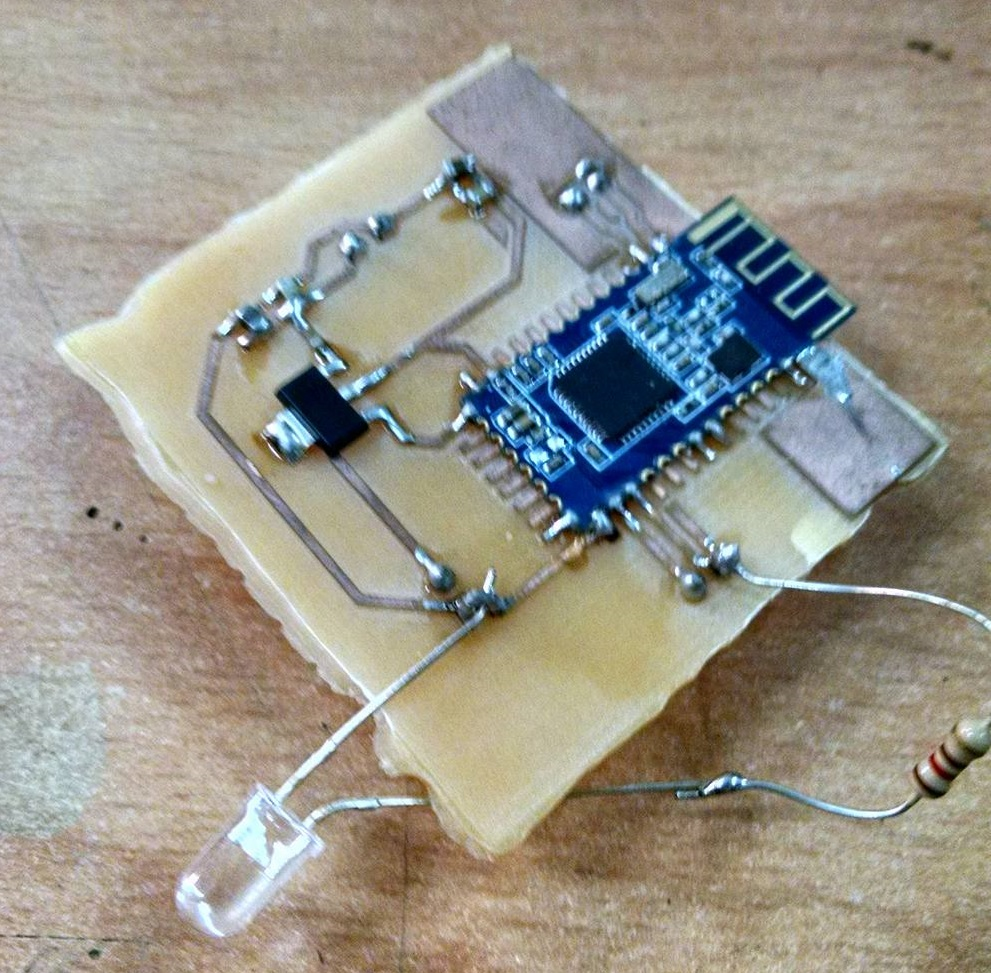
\includegraphics[width=0.5\textwidth]{keydraft}
		\caption[Mạch thử nghiệm]{Mạch thử nghiệm}
		\label{fig: keydraft}
	\end{figure}

Kết quả thử nghiệm giao tiếp và các thiết bị IO hoạt động tốt nên tiến hành đặt mạch và làm mạch chính thức ở hình \ref{fig: key1} và \ref{fig: key2}

	\begin{figure}[H]
		\centering    
		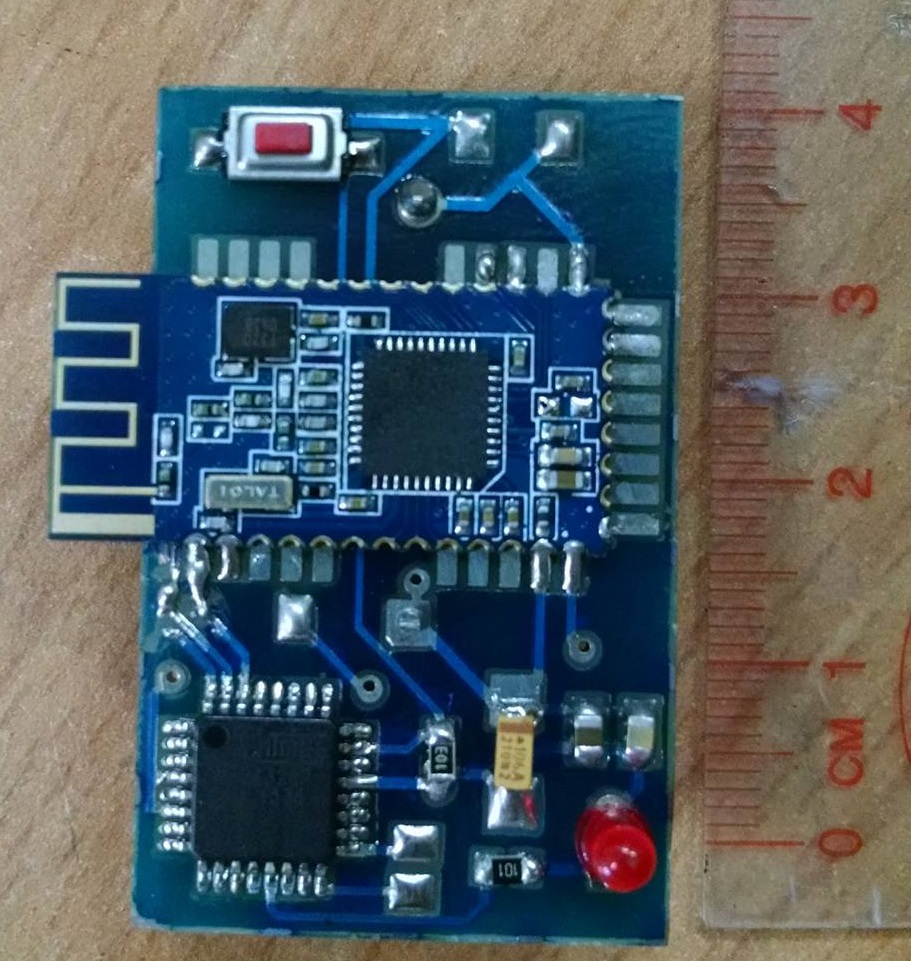
\includegraphics[width=0.5\textwidth]{key1}
		\caption[Mặt trước mạch thiết bị]{Mặt trước mạch thiết bị}
		\label{fig: key1}
	\end{figure}	
	
	\begin{figure}[H]
		\centering    
		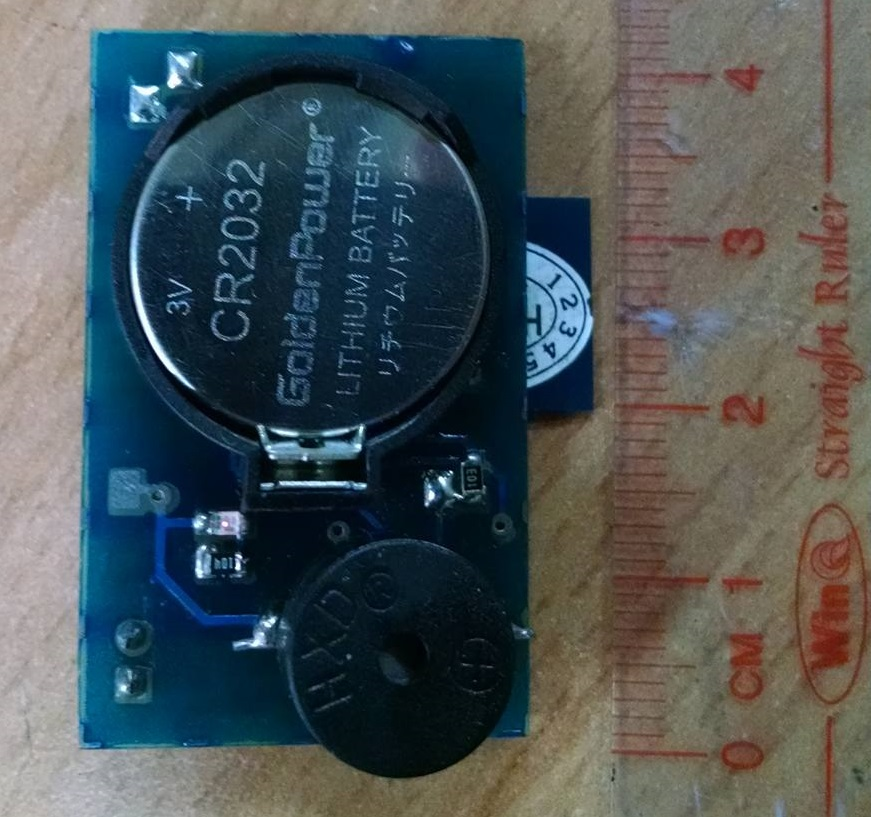
\includegraphics[width=0.5\textwidth]{key2}
		\caption[Mặt sau mạch thiết bị]{Mặt sau mạch thiết bị}
		\label{fig: key2}
	\end{figure}	
	
\subsection{Lập trình firmware cho thiết bị}

Tận dụng tính đơn giản của sản phẩm ứng dụng, các chức năng của sản phẩm được lập trình sao cho việc xử lí các input và output được thực hiện hoàn toàn bằng interrupt. Như vậy, ta sẽ không cần hiện thực thêm chương trình chính và có thể đưa vi điều khiển vào chế độ sleep mode, cụ thể hơn là Idle mode. Từ đó giúp hệ thống tiết kiệm năng lượng hơn.

	\begin{figure}[H]
		\centering    
		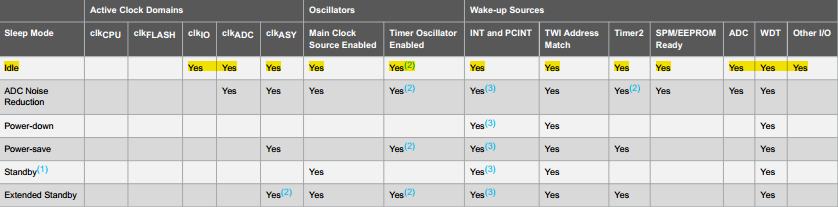
\includegraphics[width=1\textwidth]{sleep}
		\caption[Các chế độ sleep mode khác nhau và khả năng hoạt động của từng chế độ]{Các chế độ sleep mode khác nhau và khả năng hoạt động của từng chế độ}
		\label{fig: sleep}
	\end{figure}
		
Khi MCU đi vào Idle mode, CPU sẽ ngừng hoạt động nhưng các bộ USART, SPI, Timer/Counters, hệ thống Interrupt vẫn sẽ tiếp tục hoạt động.
Idle mode cho phép MCU ‘wake up’ khi xảy ra ngắt ngoài cũng như ngắt trong từ USART Receive, Timer Overflow…

\textbf{Hiện thực interrupt}

Như được đề cập ở trên, việc hiện thực chương trình cho ứng dụng cũng là hiện thực việc xử lí ở các interrupt, bao gồm USART Receive Interrupt và External Inerrupt.

\textbf{USART Receive Interrupt}

\textit{Xảy ra khi nhận được dữ liệu bất kì từ UART:} Dữ liệu này vi điều khiển nhận được thông qua module Bluetooth gửi từ thiết bị di động. Nếu dữ liệu nhận được là ‘R’, chương trình sẽ cho active chân kết nối với chuông. Nếu dữ liệu nhận được là ‘L’, chương trình cho active chân kết nối đến đèn. Ngoài ra, chương trình sẽ không có phản hồi nào khác. Chức năng trên được biểu diễn dưới dạng code:
	\begin{figure}[H]
		\centering    
		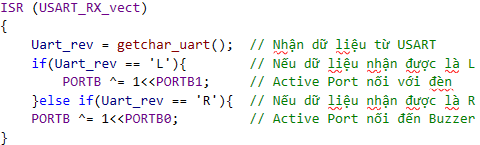
\includegraphics[width=1\textwidth]{int}
		\label{fig: int}
	\end{figure}
	
\textbf{External Inerrupt}

\textit{Xảy ra khi nhận input từ nút nhấn hoặc tín hiệu disconnect từ module Bluetooth):}
Mỗi khi có interrupt từ nút nhấn, chương trình sẽ cho truyền kí tự ‘R’ đến module Bluetooth, từ đó truyền đến thiết bị di động để phát lệnh đỗ chuông.
Khi có interrupt từ module Bluetooth, việc này xảy ra chỉ khi có 1 thiết bị đang kết nối với module Bluetooth đột nhiên mất kết nối. Khi đó, chương trình sẽ điều khiển chân kết nối với chuông để phát tín hiệu mất kết nối được thể hiện bằng đoạn code:

	\begin{figure}[H]
		\centering    
		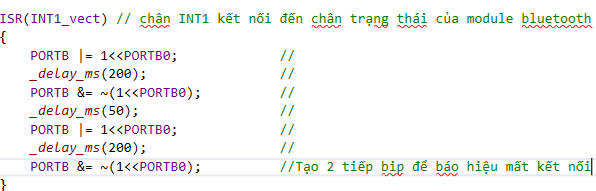
\includegraphics[width=0.8\textwidth]{int2}
		\label{fig: int2}
	\end{figure}

\textbf{Tùy chình baudrate}

Do tính chất hoạt động của sản phẩm đơn giản, hàm lượng dữ liệu truyền nhận giữa các thiết bị ít và không cần đòi hỏi tốc độ quá nhanh, việc hạ thấp baudrate sẽ giúp sản phẩm tiết kiệm năng lượng hơn. Thực tế, mỗi lần cho phát 1 lệnh bất kì giữa 2 thiết bị (smart keyring và tb di động) thì một bên chỉ truyền 1 kí tự (‘L’, ‘R’) để cho biết bên nhận phải phát sáng đèn hay  đỗ chuông. Vì lí do đó, nhóm quyết định hạ thấp baudrate đến mức nhỏ nhất mà module Bluetooth cho phép: 2400Hz
Việc điều chỉnh baudrate cho module Bluetooth khá đơn giản, chỉ cần gửi lệnh theo đúng cú pháp AT+BAUD?
Giá trị thay vào ? sẽ tương ứng với tần số mình cần điều chỉnh

	\begin{figure}[H]
		\centering    
		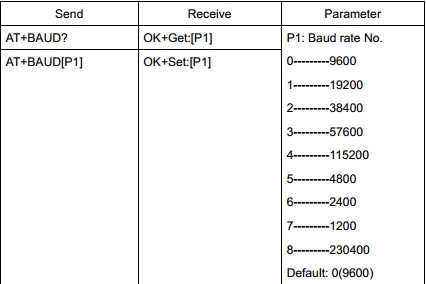
\includegraphics[width=0.7\textwidth]{baud}
		\label{fig: baud}
	\end{figure}

Như vậy, ta chỉ cần gửi lệnh \textbf{AT+BAUD6}. Nếu module Bluetooth phản hồi lại bằng lệnh OK+SET:6 thì ta đã thiết lập thành công \textbf{Baudrate 2400} cho thiết bị

Điều chỉnh tần số xung clock hoạt động của vi điều khiển.
Tốc độ xử lí càng nhanh thì đi đôi với việc tiêu tốn năng lượng càng nhiều. Để hạn chế điều này, nhóm tìm cách hạ thấp tầng số xung clock hoạt động của vi điều khiển đến mức thấp nhất có thể (128KHz). Và với công việc chính của vi điều khiển là giao tiếp UART ở tần số 2400, thì tầng số xung clock này hoàn toàn có thể đáp ứng được theo công thức sau: 

\textbf{UBRRn = FOSC/(16BAUD) – 1}

\textit{UBRRn}: giá trị cần tính để gán vào thanh ghi

\textit{FOSC}: tần số xung clock hoạt động của vi điều khiển

\textit{BAUD}: Baud rate hoạt động khi truyền nhận USART

Thay các giá trị cần tính vào ta được:

\textbf{UBRRn = 128000/(16*2400)-1 = 2.33 > 0}

Do đó việc sử dụng tần số xung clock thấp nhất (128KHz) là hoàn toàn hợp lí, đảm bảo được việc truyền nhận UART trong khi tiết kiệm năng lượng đáng kể so với việc sử dụng tần số cao hơn.
\section{Hiện thực ứng dụng di động trên Android}

\subsection{Các khái niệm trong lập trình BLE trên Android}
\label{sec: bleterm}
Dưới đây là những khái niệm chính về BLE được sử dụng: \cite{deva}

\textbf{Generic Attribute Profile (GATT) -  Cấu hình thuộc tính chung }— Cấu hình GATT là đặc điểm kỹ thuật chung cho việc truyền nhận các gói dữ liệu nhỏ được biết đến như là các "đặc tính" trên đường truyền BLE. Tất cả các cấu hình ứng dụng BLE đều dựa trên GATT.

\textbf{Attribute Protocol (ATT) - Thuộc tính của giao thức}—GATT được xây dựng bên trên lớp ATT, thường được nhắc đến là GATT/ATT. ATT được tối ưu hóa trên các thiết bị BLE và sử dụng ít dữ liệu nhất có thể. Các thuộc tính này được định danh duy nhất bởi Universally Unique Identifier (UUID), là 1 chuỗi định danh dưới chuẩn 128-bit để định danh thông tin duy nhất. Các thuộc tính được truyền bởi ATT được định dạng dưới các characteristics và services.

\textbf{Characteristic -  Đặc tính}— Bao gồm một giá trị và 0-n các khóa để miêu tả giá trị của đặc tính. Một đặc tính có thể xem như là 1 kiểu tương tự như lớp.

\textbf{Descriptor - Khóa mô tả}— Khoá mô tả được xác định để miêu tả giá trị đặc tính. Thí dụ, một khóa mô tả có thể đọc được bởi con người, thuộc phạm vi giá trị của đặc tính hoặc một giá trị đo cụ thể của một giá trị đặc tính nào đó.

\textbf{Service - Dịch vụ}— Service là một gói tổng hợp các đặc tính. Ví dụ, ta có thể có dịch vụ gọi là "Theo dõi nhịp tim" vừa bao gồm các đặc tính như "đo nhịp tim". Danh sách các cấu hình GATT và dịch vụ có thể tìm thấy tại bluetooth.org.

\subsection{Phát triển ứng dụng Android}
%TODO: bổ sung hình giao diện ứng dụng
Ứng dụng Android được phát triển từ nguồn ứng dụng mở android-BluetoothLeGatt\cite{blegatt} được cung cấp bởi Google. Ứng dụng này có chức năng demo thiết lập kết nối và nhận dữ liệu theo chuẩn BLE.

Nhóm chúng tôi trong quá trình tìm hiểu đã nhận thấy phù hợp với đề tài và có thể phát triển chức năng cảnh báo khi mất kết nối và báo hiệu để thiết bị Smart Keyring kích hoạt buzzer/led.

%TODO: bỏ các file code và chức năng

Ứng dụng lập trình dựa theo 4 file chính:

\textit{DeviceScanActivity.java:} chức năng tìm kiếm và hiện thị thiết bị BLE

\textit{DeviceControlActivity.java:} chức năng quản lý kết nối và hiển thị các thông tin về trạng thái kết nối và các service đang có.

\textit{BluetoothLeService.java:} quản lý và điều khiển các service

Cơ chế hoạt động của lệnh gửi ký tự qua BLE trên Android:

\begin{lstlisting}
	// BluetoothLeService.java
    public void ring(){
	    char sendC = 'R'; // gan ky tu can gui la 'R'
	    mGattCharacteristics.setValue(String.valueOf(sendC)); // gan ky tu can gui cho characteristic
	    mBluetoothGatt.writeCharacteristic(mGattCharacteristics); // gui ky tu thong qua GATT BLE
	    Log.d("Ring function Call", "Service");
    }
\end{lstlisting}

Xử lý khi mất kết nối: các hoạt động khi kết nối và mất kết nối được quản lý với \textbf{BroadcastReceiver()} bao gồm các giá trị \textbf{BluetoothLeService}. Khi các giá trị này thay đổi thì sẽ dẫn tới các hoạt động tương ứng:

\begin{lstlisting}
	// DeviceControlActivity.java
 BroadcastReceiver() {
  	@Override
  	public void onReceive(Context context, Intent intent) {
  		if (BluetoothLeService.ACTION_GATT_CONNECTED.equals(action)) {
  			mConnected = true;
  			updateConnectionState(R.string.connected);
  			invalidateOptionsMenu();
  		} else if (BluetoothLeService.ACTION_GATT_DISCONNECTED.equals(action)){
	  		mp=MediaPlayer.create(this,R.raw.noti);
	  		mp.start();
  		}
	};
\end{lstlisting}
Và giao diện ứng dụng được thiết kế:

	\begin{figure}[H]
		\centering    
		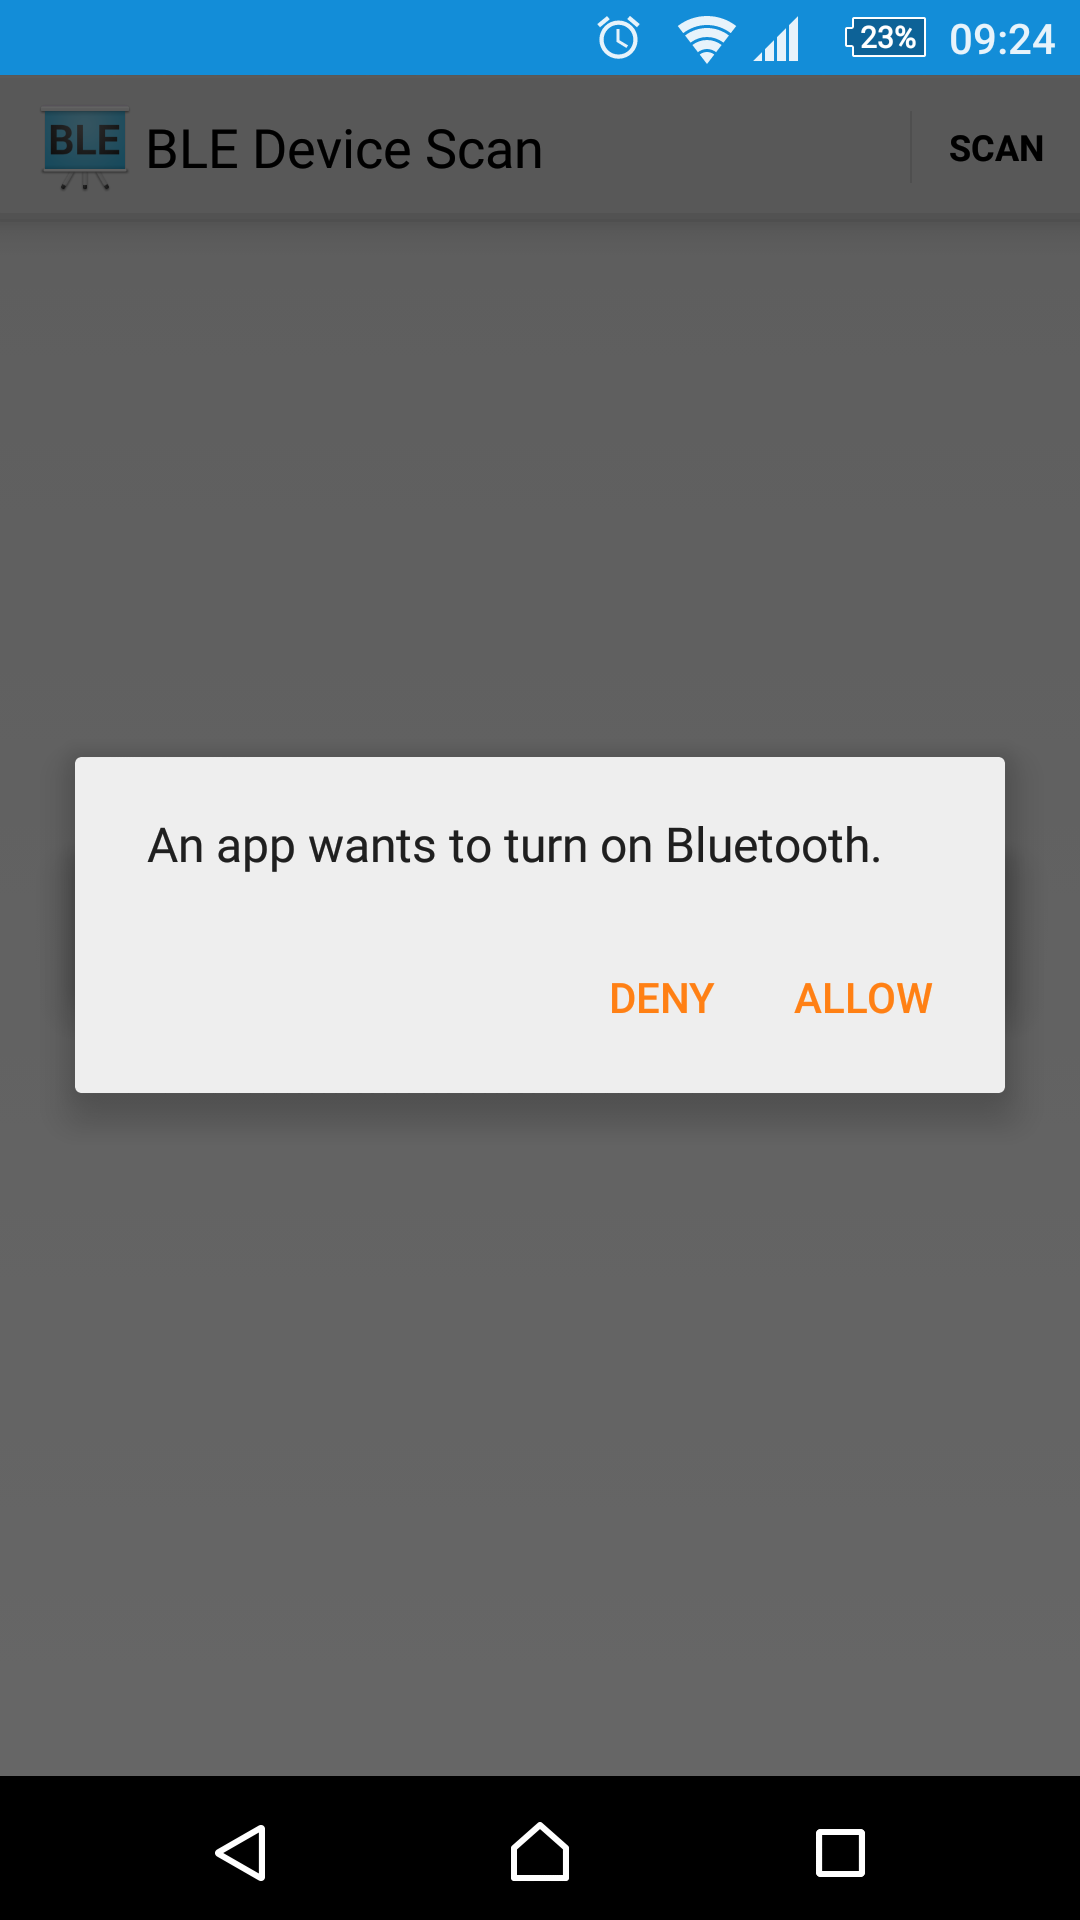
\includegraphics[width=0.6\textwidth]{androidoff}
		\caption[Giao diện kiểm tra BLE]{Giao diện kiểm tra BLE}
		\label{fig: androidoff}
	\end{figure}
Khi khởi động ứng dụng di động, chương trình sẽ kiểm tra thiết bị di động đã bật chế độ Bluetooth chưa và chọn để bắt đầu sử dụng như hình \ref{fig: androidoff}

Nếu thiết bị di động đã bật sẵn chế độ kết nối Bluetooth thì giao diện \ref{fig: androidoff} sẽ không hiện ra.

	\begin{figure}[H]
		\centering    
		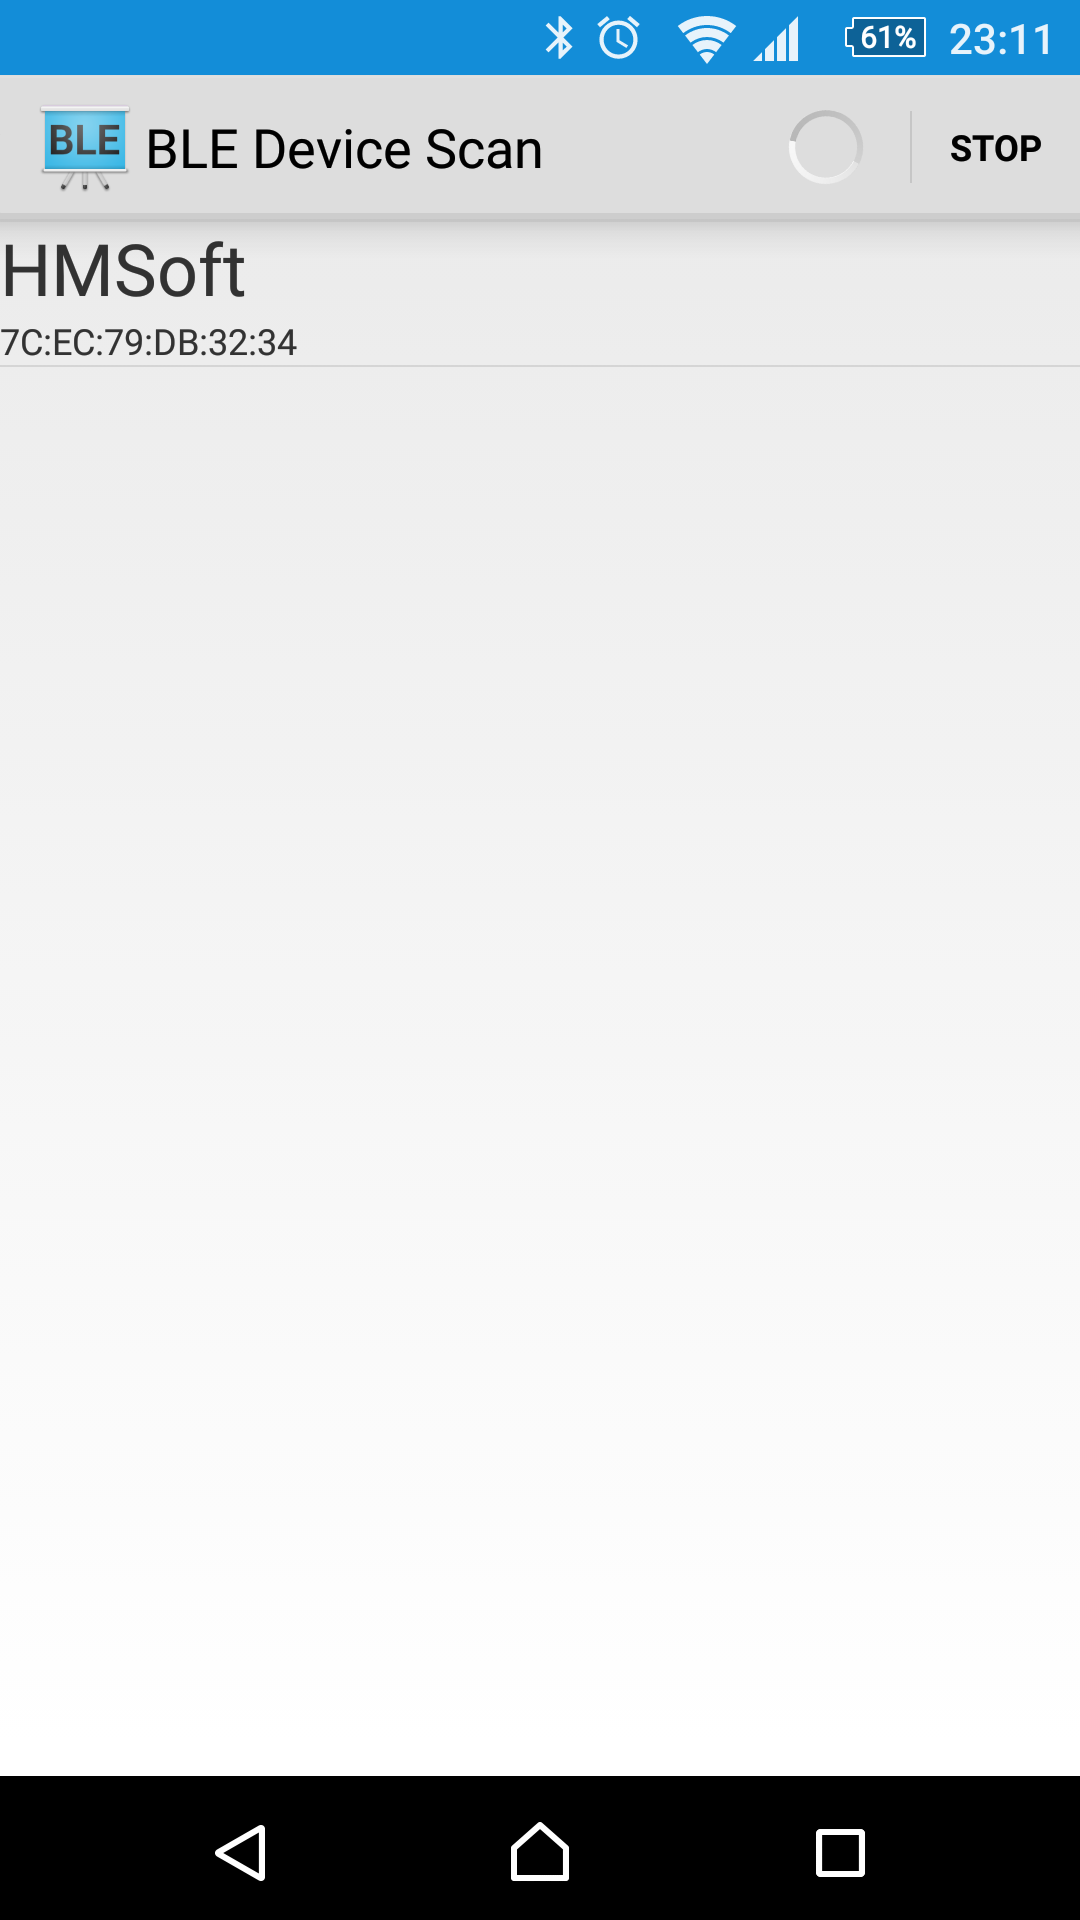
\includegraphics[width=0.6\textwidth]{android1}
		\caption[Giao diện scan thiết bị BLE]{Giao diện scan thiết bị BLE}
		\label{fig: android1}
	\end{figure}
Sau đó ta chọn thiết bị BLE để kết nối, ở đây thiết bị Smart Keyring sử dụng module HM-10 với thiết lập tên hiển thị mặc định là HMSoft. 
	\begin{figure}[H]
		\centering    
		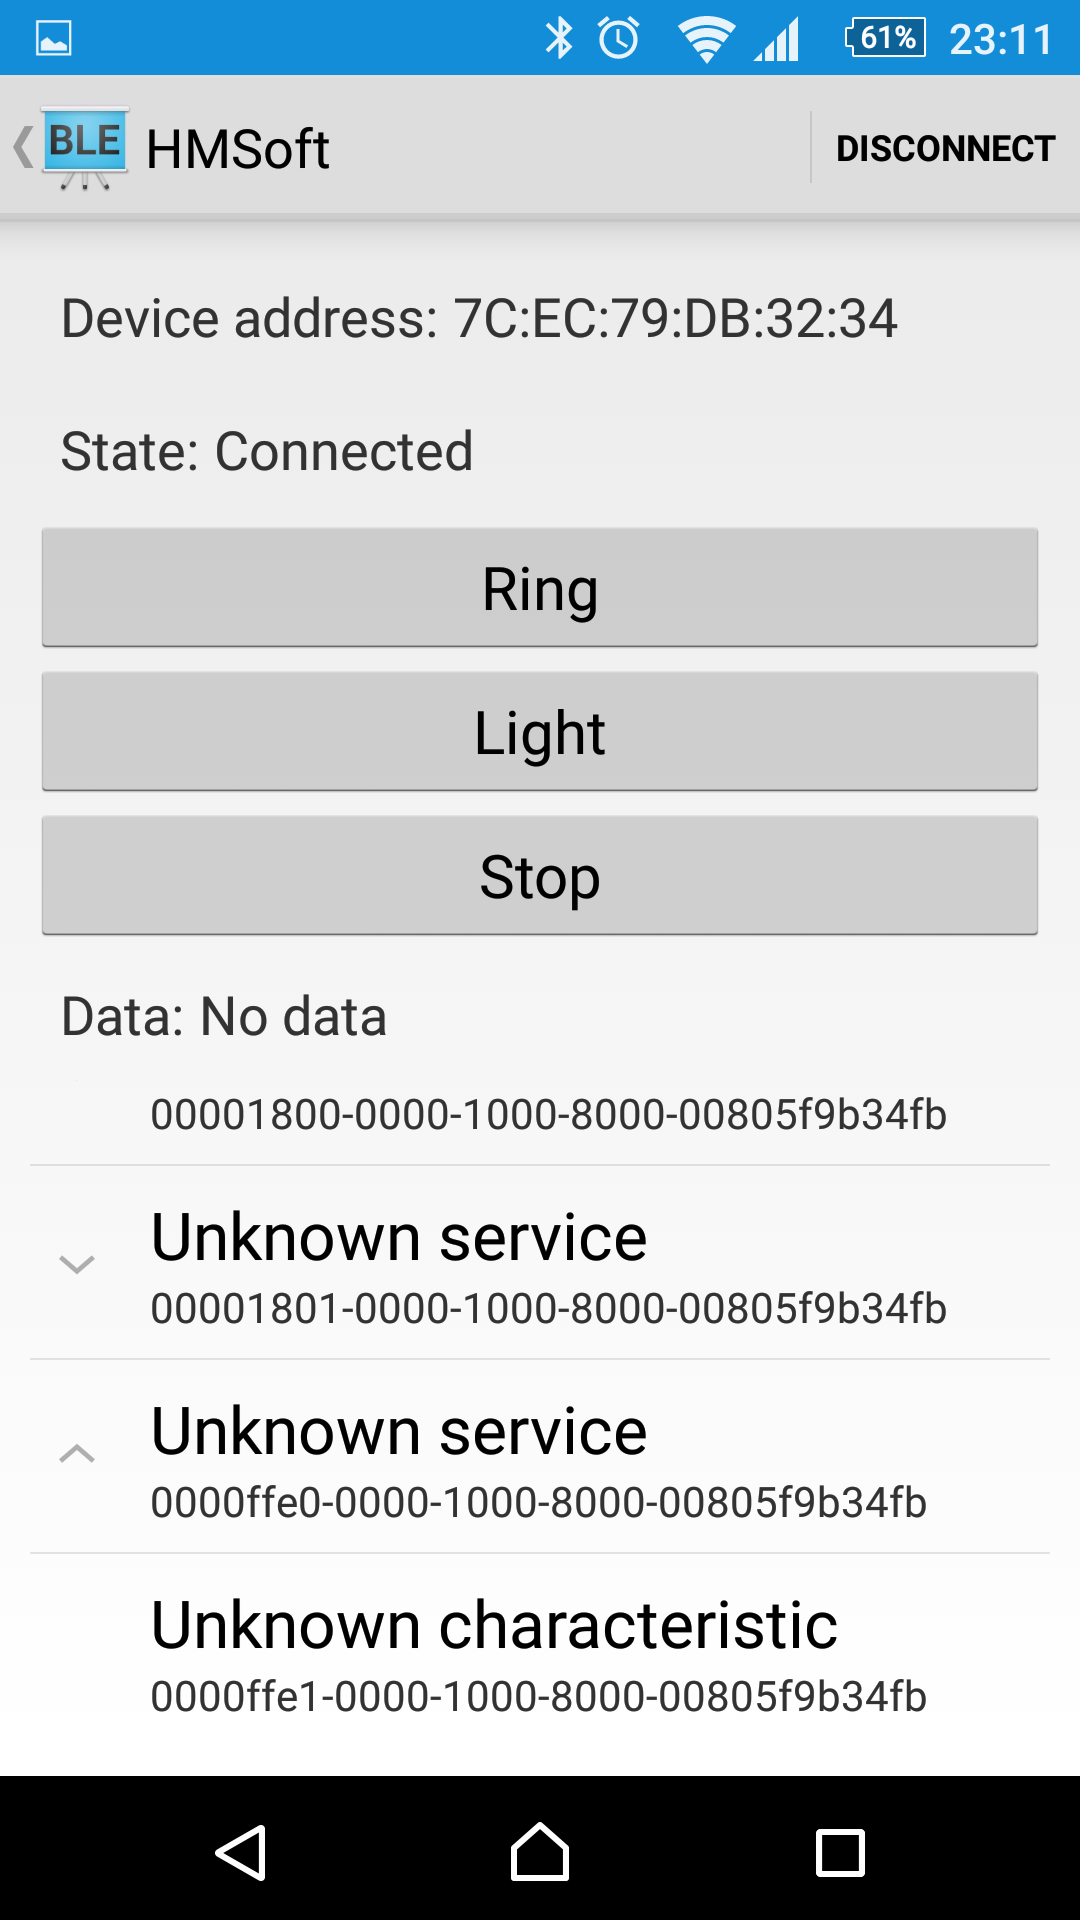
\includegraphics[width=0.6\textwidth]{android2}
		\caption[Giao diện chính của ứng dụng di động]{Giao diện chính của ứng dụng di động}
		\label{fig: android2}
	\end{figure}
	
	Sau khi kết nối, chúng ta sẽ có những thông tin như:
	
	• Device address: địa chỉ MAC của chip CC2540/2541.
	
	• State: Connected hoặc Disconnected -  báo trạng thái kết nối giữa ứng dụng và thiết bị.
	
	• Các service là các characteristic (xem thêm tại \ref{sec: bleterm} ): vì ứng dụng di động đang trong quá trình tìm hiểu và phát triển nên hiển thị các uuid để dễ theo dõi.
	
	Ngoài ra còn có các nút chức năng:
	
	• Ring: gửi yêu cầu bật/tắt báo hiệu bằng buzzer tới thiết bị Smart Keyring.
	
	• Light: gửi yêu cầu bật/tắt báo hiệu bằng LED tới thiết bị Smart Keyring.
	
	• Stop: tắt báo hiệu bằng âm thanh trên thiết bị di động sau khi mất kết nối với thiết bị Smart Keyring.
	
	Để sử dụng các chức năng trên, ta cần chọn service \textbf{0000ffe0-0000-1000-8000-00805f9b34fb} và characteristic \textbf{0000ffe1-0000-1000-8000-00805f9b34fb} - tức là service và characteristic của chức năng đọc truyền nhận dữ liệu thông qua kết nối Bluetooth.

\textit{Source code có thể xem tại: } https://github.com/MrWhoz/ble-smartlkey
	%Demo ứng dụng và đề tài xem thêm tại: 
	%TODO: bỏ link utube
\chapter{Thử nghiệm và đánh giá kết quả đạt được}

% **************************** Define Graphics Path **************************
\ifpdf
    \graphicspath{{Chapter3/Figs/Raster/}{Chapter3/Figs/PDF/}{Chapter3/Figs/}}
\else
    \graphicspath{{Chapter3/Figs/Vector/}{Chapter3/Figs/}}
\fi

\section{Thử nghiệm}
\subsection{Khoảng cách hoạt động}

\textbf{Phương pháp thực nghiệm:} Kết nối thiết bị Smart Keyring và thiết bị di động, liên tuc kiểm tra kết nối trao đổi tín hiệu giữa 2 thiết bị và tăng dần khoảng khoảng cách cho đến khi có báo hiệu mất kết nối. Thực nghiệm ở 2 trường hợp môi trường không vật cản và có vật cản.

Thử nghiệm được thực hiện với điện thoại Sony Xperia Z1:

\begin{table}[!ht]
	\centering
	\begin{tabular}{|c | c|}
		\hline 
		Các lần đo & Khoảng cách còn hoạt động  \\ 
		\hline
		Lần 1 & 22m \\
		
		Lần 2 &	22m \\
		
		Lần 3 &	21.5m \\
		
		Lần 4 &	23m \\
		
		Lần 5 &	23m \\
		
		Lần 6 &	22.5m \\
		
		Lần 7 &	22m \\
		
		Lần 8 &	21m \\
		
		Lần 9 &	22m \\
		
		Lần 10 & 22m \\		
		
		\hline 		
	\end{tabular}
	\caption{Thử nghiệm khoảng cách hoạt động khi không có vật cản}		
	\label{table:distance-no}
\end{table}

\begin{table}[!ht]
	\centering
	\begin{tabular}{|c | c|}
		\hline 
		 Các lần đo & Khoảng cách còn hoạt động  \\ 
		\hline
		Lần 1 &	8m \\
		
		Lần 2 &	8m \\
		
		Lần 3 &	8.5m \\
		
		Lần 4 &	8.5m \\
		
		Lần 5 &	8m \\
		
		Lần 6 &	7.5m \\
		
		Lần 7 &	8m \\
		
		Lần 8 &	7.5m \\
		
		Lần 9 &	8m \\
		
		Lần 10 & 8.5m \\		
		\hline 		
	\end{tabular}
\caption{Thử nghiệm khoảng cách hoạt động khi có vật cản}		
\label{table:distance}
\end{table}

Thực nghiệm cho thấy, phạm vi tối đa trung bình để việc truyền nhận dữ liệu còn chính xác là vào khoảng 22m đối với môi trường không vật cản, 8m đối với môi trường có vật cản( các 1 bức tường).

\newpage
\subsection{Năng lượng tiêu thụ}
Thông số tiêu thụ năng lượng của các linh kiện kiện theo nhà sản xuất:

• Tiêu thụ của HM-10: 0.2mA ở sleep mode, 8mA ở active mode

• Tiêu thụ của vi điều khiển ATmega328P: 0.2mA ở active mode

• Tiêu thụ của đèn LED: 

• Buzzer tín hiệu khi kích hoạt: 32mA

• Dung lượng nguồn sử dụng: Pin CR2032 dung lượng 220mAh

Thực tế năng lượng tiêu thụ:

\textbf{Phương pháp thực nghiệm:} kết nối thiết bị Smart Keyring với thiết bị di động, mỗi ngày kiểm tra kết nối 2 lần vào lúc 7h sáng và 5h chiều và tự đưa về chế độ Idle ở thời gian rảnh. Giữ thiết bị hoạt động liên tục với pin CR2032 cho đến khi hết pin.

\textbf{Kết quả: } Bắt đầu thực nghiệm vào lúc 7h sáng ngày 1/11, thiết bị không còn khả năng kết nối vào lúc 4h30 chiều ngày 18/11 mặc dù đèn nguồn vẫn còn sáng nhưng không đủ năng lượng để duy trì module BLE giữ kết nối.

\section{Đánh giá kết quả ứng dụng thực tế}
\label{result}
Phần này sẽ đánh giá về khả năng ứng dụng thực tế dựa trên kết quả thực nghiệm.

Về khoảng cách hoạt động tối đa và tính ứng dụng thực tế hiệu quả:

• \textbf{Môi trường không vật cản vào khoảng 22m: }hiệu quả trong việc báo mất kết nối trong các trường hợp thực tế như bỏ quên chìa khóa trên xe trong bãi giữ xe, thiết bị di động tại nơi công cộng vì khoảng cách hợp lý không quá ngắn và cũng như không quá xa.

• \textbf{Môi trường có vật cản vào khoảng 8m:} hiệu quả trong việc báo mất kết nối trong các trường hợp thực tế như để quên trong phòng, báo hiệu sớm để người dùng có thể biết ngay khi bỏ quên 1 trong 2 thiết bị khi vừa rời khỏi phòng. Và khoảng cách đủ để duy trì kết nối kích hoạt chế độ báo hiệu tìm kiếm khi thiết bị che khuất tầm nhìn giúp việc tìm kiếm nhanh chóng và hiệu quả hơn.

Về thời gian hoạt động: vì hạn chế trong việc không tối ưu thiết bị, đạt 18 ngày thay pin 1 lần là kết quả kém hiệu quả trong cuộc sống hằng ngày.
\chapter{My fourth chapter}

% **************************** Define Graphics Path **************************
\ifpdf
    \graphicspath{{Chapter3/Figs/Raster/}{Chapter3/Figs/PDF/}{Chapter3/Figs/}}
\else
    \graphicspath{{Chapter3/Figs/Vector/}{Chapter3/Figs/}}
\fi

\section{First section of the fourth chapter}
And now I begin my third chapter here \dots

And now to cite some more people~\citet{Rea85,Ancey1996}

\subsection{First subsection in the first section}
\dots and some more 

\subsection{Second subsection in the first section}
\dots and some more \dots

\subsubsection{First subsub section in the second subsection}
\dots and some more in the first subsub section otherwise it all looks the same
doesn't it? well we can add some text to it \dots

\subsection{Third subsection in the first section}
\dots and some more \dots

\subsubsection{First subsub section in the third subsection}
\dots and some more in the first subsub section otherwise it all looks the same
doesn't it? well we can add some text to it and some more and some more and
some more and some more and some more and some more and some more \dots

\subsubsection{Second subsub section in the third subsection}
\dots and some more in the first subsub section otherwise it all looks the same
doesn't it? well we can add some text to it \dots

\section{Second section of the third chapter}
and here I write more \dots

\section{The layout of formal tables}
This section has been modified from ``Publication quality tables in \LaTeX*''
 by Simon Fear.

The layout of a table has been established over centuries of experience and 
should only be altered in extraordinary circumstances. 

When formatting a table, remember two simple guidelines at all times:

\begin{enumerate}
  \item Never, ever use vertical rules (lines).
  \item Never use double rules.
\end{enumerate}

These guidelines may seem extreme but I have
never found a good argument in favour of breaking them. For
example, if you feel that the information in the left half of
a table is so different from that on the right that it needs
to be separated by a vertical line, then you should use two
tables instead. Not everyone follows the second guideline:

There are three further guidelines worth mentioning here as they
are generally not known outside the circle of professional
typesetters and subeditors:

\begin{enumerate}\setcounter{enumi}{2}
  \item Put the units in the column heading (not in the body of
          the table).
  \item Always precede a decimal point by a digit; thus 0.1
      {\em not} just .1.
  \item Do not use `ditto' signs or any other such convention to
      repeat a previous value. In many circumstances a blank
      will serve just as well. If it won't, then repeat the value.
\end{enumerate}

A frequently seen mistake is to use `\textbackslash begin\{center\}' \dots `\textbackslash end\{center\}' inside a figure or table environment. This center environment can cause additional vertical space. If you want to avoid that just use `\textbackslash centering'


\begin{table}
\caption{A badly formatted table}
\centering
\label{table:bad_table}
\begin{tabular}{|l|c|c|c|c|}
\hline 
& \multicolumn{2}{c}{Species I} & \multicolumn{2}{c|}{Species II} \\ 
\hline
Dental measurement  & mean & SD  & mean & SD  \\ \hline 
\hline
I1MD & 6.23 & 0.91 & 5.2  & 0.7  \\
\hline 
I1LL & 7.48 & 0.56 & 8.7  & 0.71 \\
\hline 
I2MD & 3.99 & 0.63 & 4.22 & 0.54 \\
\hline 
I2LL & 6.81 & 0.02 & 6.66 & 0.01 \\
\hline 
CMD & 13.47 & 0.09 & 10.55 & 0.05 \\
\hline 
CBL & 11.88 & 0.05 & 13.11 & 0.04\\ 
\hline 
\end{tabular}
\end{table}

\begin{table}
\caption{A nice looking table}
\centering
\label{table:nice_table}
\begin{tabular}{l c c c c}
\hline 
\multirow{2}{*}{Dental measurement} & \multicolumn{2}{c}{Species I} & \multicolumn{2}{c}{Species II} \\ 
\cline{2-5}
  & mean & SD  & mean & SD  \\ 
\hline
I1MD & 6.23 & 0.91 & 5.2  & 0.7  \\

I1LL & 7.48 & 0.56 & 8.7  & 0.71 \\

I2MD & 3.99 & 0.63 & 4.22 & 0.54 \\

I2LL & 6.81 & 0.02 & 6.66 & 0.01 \\

CMD & 13.47 & 0.09 & 10.55 & 0.05 \\

CBL & 11.88 & 0.05 & 13.11 & 0.04\\ 
\hline 
\end{tabular}
\end{table}


\begin{table}
\caption{Even better looking table using booktabs}
\centering
\label{table:good_table}
\begin{tabular}{l c c c c}
\toprule
\multirow{2}{*}{Dental measurement} & \multicolumn{2}{c}{Species I} & \multicolumn{2}{c}{Species II} \\ 
\cmidrule{2-5}
  & mean & SD  & mean & SD  \\ 
\midrule
I1MD & 6.23 & 0.91 & 5.2  & 0.7  \\

I1LL & 7.48 & 0.56 & 8.7  & 0.71 \\

I2MD & 3.99 & 0.63 & 4.22 & 0.54 \\

I2LL & 6.81 & 0.02 & 6.66 & 0.01 \\

CMD & 13.47 & 0.09 & 10.55 & 0.05 \\

CBL & 11.88 & 0.05 & 13.11 & 0.04\\ 
\bottomrule
\end{tabular}
\end{table}

%\chapter{My fifth chapter}

% **************************** Define Graphics Path **************************
\ifpdf
    \graphicspath{{Chapter3/Figs/Raster/}{Chapter3/Figs/PDF/}{Chapter3/Figs/}}
\else
    \graphicspath{{Chapter3/Figs/Vector/}{Chapter3/Figs/}}
\fi

\section{First section of the fifth chapter}
And now I begin my third chapter here \dots

And now to cite some more people~\citet{Rea85,Ancey1996}

\subsection{First subsection in the first section}
\dots and some more 

\subsection{Second subsection in the first section}
\dots and some more \dots

\subsubsection{First subsub section in the second subsection}
\dots and some more in the first subsub section otherwise it all looks the same
doesn't it? well we can add some text to it \dots

\subsection{Third subsection in the first section}
\dots and some more \dots

\subsubsection{First subsub section in the third subsection}
\dots and some more in the first subsub section otherwise it all looks the same
doesn't it? well we can add some text to it and some more and some more and
some more and some more and some more and some more and some more \dots

\subsubsection{Second subsub section in the third subsection}
\dots and some more in the first subsub section otherwise it all looks the same
doesn't it? well we can add some text to it \dots

\section{Second section of the third chapter}
and here I write more \dots

\section{The layout of formal tables}
This section has been modified from ``Publication quality tables in \LaTeX*''
 by Simon Fear.

The layout of a table has been established over centuries of experience and 
should only be altered in extraordinary circumstances. 

When formatting a table, remember two simple guidelines at all times:

\begin{enumerate}
  \item Never, ever use vertical rules (lines).
  \item Never use double rules.
\end{enumerate}

These guidelines may seem extreme but I have
never found a good argument in favour of breaking them. For
example, if you feel that the information in the left half of
a table is so different from that on the right that it needs
to be separated by a vertical line, then you should use two
tables instead. Not everyone follows the second guideline:

There are three further guidelines worth mentioning here as they
are generally not known outside the circle of professional
typesetters and subeditors:

\begin{enumerate}\setcounter{enumi}{2}
  \item Put the units in the column heading (not in the body of
          the table).
  \item Always precede a decimal point by a digit; thus 0.1
      {\em not} just .1.
  \item Do not use `ditto' signs or any other such convention to
      repeat a previous value. In many circumstances a blank
      will serve just as well. If it won't, then repeat the value.
\end{enumerate}

A frequently seen mistake is to use `\textbackslash begin\{center\}' \dots `\textbackslash end\{center\}' inside a figure or table environment. This center environment can cause additional vertical space. If you want to avoid that just use `\textbackslash centering'


\begin{table}
\caption{A badly formatted table}
\centering
\label{table:bad_table}
\begin{tabular}{|l|c|c|c|c|}
\hline 
& \multicolumn{2}{c}{Species I} & \multicolumn{2}{c|}{Species II} \\ 
\hline
Dental measurement  & mean & SD  & mean & SD  \\ \hline 
\hline
I1MD & 6.23 & 0.91 & 5.2  & 0.7  \\
\hline 
I1LL & 7.48 & 0.56 & 8.7  & 0.71 \\
\hline 
I2MD & 3.99 & 0.63 & 4.22 & 0.54 \\
\hline 
I2LL & 6.81 & 0.02 & 6.66 & 0.01 \\
\hline 
CMD & 13.47 & 0.09 & 10.55 & 0.05 \\
\hline 
CBL & 11.88 & 0.05 & 13.11 & 0.04\\ 
\hline 
\end{tabular}
\end{table}

\begin{table}
\caption{A nice looking table}
\centering
\label{table:nice_table}
\begin{tabular}{l c c c c}
\hline 
\multirow{2}{*}{Dental measurement} & \multicolumn{2}{c}{Species I} & \multicolumn{2}{c}{Species II} \\ 
\cline{2-5}
  & mean & SD  & mean & SD  \\ 
\hline
I1MD & 6.23 & 0.91 & 5.2  & 0.7  \\

I1LL & 7.48 & 0.56 & 8.7  & 0.71 \\

I2MD & 3.99 & 0.63 & 4.22 & 0.54 \\

I2LL & 6.81 & 0.02 & 6.66 & 0.01 \\

CMD & 13.47 & 0.09 & 10.55 & 0.05 \\

CBL & 11.88 & 0.05 & 13.11 & 0.04\\ 
\hline 
\end{tabular}
\end{table}


\begin{table}
\caption{Even better looking table using booktabs}
\centering
\label{table:good_table}
\begin{tabular}{l c c c c}
\toprule
\multirow{2}{*}{Dental measurement} & \multicolumn{2}{c}{Species I} & \multicolumn{2}{c}{Species II} \\ 
\cmidrule{2-5}
  & mean & SD  & mean & SD  \\ 
\midrule
I1MD & 6.23 & 0.91 & 5.2  & 0.7  \\

I1LL & 7.48 & 0.56 & 8.7  & 0.71 \\

I2MD & 3.99 & 0.63 & 4.22 & 0.54 \\

I2LL & 6.81 & 0.02 & 6.66 & 0.01 \\

CMD & 13.47 & 0.09 & 10.55 & 0.05 \\

CBL & 11.88 & 0.05 & 13.11 & 0.04\\ 
\bottomrule
\end{tabular}
\end{table}

%\include{Chapter6/chapter6}
%\include{Chapter7/chapter7}



% ********************************** Back Matter *******************************
% Backmatter should be commented out, if you are using appendices after References
%\backmatter

% ********************************** Bibliography ******************************
\begin{spacing}{0.9}

% To use the conventional natbib style referencing
% Bibliography style previews: http://nodonn.tipido.net/bibstyle.php
% Reference styles: http://sites.stat.psu.edu/~surajit/present/bib.htm

%\bibliographystyle{apalike}
%\bibliographystyle{unsrt} % Use for unsorted references  
\bibliographystyle{plainnat} % use this to have URLs listed in References
\cleardoublepage
\bibliography{References/references} % Path to your References.bib file


% If you would like to use BibLaTeX for your references, pass `custombib' as
% an option in the document class. The location of 'reference.bib' should be
% specified in the preamble.tex file in the custombib section.
% Comment out the lines related to natbib above and uncomment the following line.

%\printbibliography[heading=bibintoc, title={References}]


\end{spacing}

%\appendix
%% ******************************* Thesis Appendix A ****************************
\chapter{How to install \LaTeX} 

\section*{Windows OS}

\subsection*{TeXLive package - full version}
\begin{enumerate}
\item	Download the TeXLive ISO (2.2GB) from\\
\href{https://www.tug.org/texlive/}{https://www.tug.org/texlive/}
\item	Download WinCDEmu (if you don't have a virtual drive) from \\
\href{http://wincdemu.sysprogs.org/download/}
{http://wincdemu.sysprogs.org/download/}
\item	To install Windows CD Emulator follow the instructions at\\
\href{http://wincdemu.sysprogs.org/tutorials/install/}
{http://wincdemu.sysprogs.org/tutorials/install/}
\item	Right click the iso and mount it using the WinCDEmu as shown in \\
\href{http://wincdemu.sysprogs.org/tutorials/mount/}{
http://wincdemu.sysprogs.org/tutorials/mount/}
\item	Open your virtual drive and run setup.pl
\end{enumerate}

or

\subsection*{Basic MikTeX - \TeX~ distribution}
\begin{enumerate}
\item	Download Basic-MiK\TeX (32bit or 64bit) from\\
\href{http://miktex.org/download}{http://miktex.org/download}
\item	Run the installer 
\item	To add a new package go to Start >> All Programs >> MikTex >> Maintenance (Admin) and choose Package Manager
\item	Select or search for packages to install
\end{enumerate}

\subsection*{TexStudio - \TeX~ editor}
\begin{enumerate}
\item	Download TexStudio from\\
\href{http://texstudio.sourceforge.net/\#downloads}
{http://texstudio.sourceforge.net/\#downloads} 
\item	Run the installer
\end{enumerate}

\section*{Mac OS X}
\subsection*{MacTeX - \TeX~ distribution}
\begin{enumerate}
\item	Download the file from\\
\href{https://www.tug.org/mactex/}{https://www.tug.org/mactex/}
\item	Extract and double click to run the installer. It does the entire configuration, sit back and relax.
\end{enumerate}

\subsection*{TexStudio - \TeX~ editor}
\begin{enumerate}
\item	Download TexStudio from\\
\href{http://texstudio.sourceforge.net/\#downloads}
{http://texstudio.sourceforge.net/\#downloads} 
\item	Extract and Start
\end{enumerate}


\section*{Unix/Linux}
\subsection*{TeXLive - \TeX~ distribution}
\subsubsection*{Getting the distribution:}
\begin{enumerate}
\item	TexLive can be downloaded from\\
\href{http://www.tug.org/texlive/acquire-netinstall.html}
{http://www.tug.org/texlive/acquire-netinstall.html}.
\item	TexLive is provided by most operating system you can use (rpm,apt-get or yum) to get TexLive distributions
\end{enumerate}

\subsubsection*{Installation}
\begin{enumerate}
\item	Mount the ISO file in the mnt directory
\begin{verbatim}
mount -t iso9660 -o ro,loop,noauto /your/texlive####.iso /mnt
\end{verbatim}

\item	Install wget on your OS (use rpm, apt-get or yum install)
\item	Run the installer script install-tl.
\begin{verbatim}
	cd /your/download/directory
	./install-tl
\end{verbatim}
\item	Enter command `i' for installation

\item	Post-Installation configuration:\\
\href{http://www.tug.org/texlive/doc/texlive-en/texlive-en.html\#x1-320003.4.1}
{http://www.tug.org/texlive/doc/texlive-en/texlive-en.html\#x1-320003.4.1} 
\item	Set the path for the directory of TexLive binaries in your .bashrc file
\end{enumerate}

\subsubsection*{For 32bit OS}
For Bourne-compatible shells such as bash, and using Intel x86 GNU/Linux and a default directory setup as an example, the file to edit might be \begin{verbatim}
edit $~/.bashrc file and add following lines
PATH=/usr/local/texlive/2011/bin/i386-linux:$PATH; 
export PATH 
MANPATH=/usr/local/texlive/2011/texmf/doc/man:$MANPATH;
export MANPATH 
INFOPATH=/usr/local/texlive/2011/texmf/doc/info:$INFOPATH;
export INFOPATH
\end{verbatim}
\subsubsection*{For 64bit OS}
\begin{verbatim}
edit $~/.bashrc file and add following lines
PATH=/usr/local/texlive/2011/bin/x86_64-linux:$PATH;
export PATH 
MANPATH=/usr/local/texlive/2011/texmf/doc/man:$MANPATH;
export MANPATH 
INFOPATH=/usr/local/texlive/2011/texmf/doc/info:$INFOPATH;
export INFOPATH

\end{verbatim}



%\subsection{Installing directly using Linux packages} 
\subsubsection*{Fedora/RedHat/CentOS:}
\begin{verbatim} 
sudo yum install texlive 
sudo yum install psutils 
\end{verbatim}


\subsubsection*{SUSE:}
\begin{verbatim}
sudo zypper install texlive
\end{verbatim}


\subsubsection*{Debian/Ubuntu:}
\begin{verbatim} 
sudo apt-get install texlive texlive-latex-extra 
sudo apt-get install psutils
\end{verbatim}

% ********************************** Appendices ********************************

\begin{appendices} % Using appendices environment for more functunality

%% ******************************* Thesis Appendix A ****************************
\chapter{How to install \LaTeX} 

\section*{Windows OS}

\subsection*{TeXLive package - full version}
\begin{enumerate}
\item	Download the TeXLive ISO (2.2GB) from\\
\href{https://www.tug.org/texlive/}{https://www.tug.org/texlive/}
\item	Download WinCDEmu (if you don't have a virtual drive) from \\
\href{http://wincdemu.sysprogs.org/download/}
{http://wincdemu.sysprogs.org/download/}
\item	To install Windows CD Emulator follow the instructions at\\
\href{http://wincdemu.sysprogs.org/tutorials/install/}
{http://wincdemu.sysprogs.org/tutorials/install/}
\item	Right click the iso and mount it using the WinCDEmu as shown in \\
\href{http://wincdemu.sysprogs.org/tutorials/mount/}{
http://wincdemu.sysprogs.org/tutorials/mount/}
\item	Open your virtual drive and run setup.pl
\end{enumerate}

or

\subsection*{Basic MikTeX - \TeX~ distribution}
\begin{enumerate}
\item	Download Basic-MiK\TeX (32bit or 64bit) from\\
\href{http://miktex.org/download}{http://miktex.org/download}
\item	Run the installer 
\item	To add a new package go to Start >> All Programs >> MikTex >> Maintenance (Admin) and choose Package Manager
\item	Select or search for packages to install
\end{enumerate}

\subsection*{TexStudio - \TeX~ editor}
\begin{enumerate}
\item	Download TexStudio from\\
\href{http://texstudio.sourceforge.net/\#downloads}
{http://texstudio.sourceforge.net/\#downloads} 
\item	Run the installer
\end{enumerate}

\section*{Mac OS X}
\subsection*{MacTeX - \TeX~ distribution}
\begin{enumerate}
\item	Download the file from\\
\href{https://www.tug.org/mactex/}{https://www.tug.org/mactex/}
\item	Extract and double click to run the installer. It does the entire configuration, sit back and relax.
\end{enumerate}

\subsection*{TexStudio - \TeX~ editor}
\begin{enumerate}
\item	Download TexStudio from\\
\href{http://texstudio.sourceforge.net/\#downloads}
{http://texstudio.sourceforge.net/\#downloads} 
\item	Extract and Start
\end{enumerate}


\section*{Unix/Linux}
\subsection*{TeXLive - \TeX~ distribution}
\subsubsection*{Getting the distribution:}
\begin{enumerate}
\item	TexLive can be downloaded from\\
\href{http://www.tug.org/texlive/acquire-netinstall.html}
{http://www.tug.org/texlive/acquire-netinstall.html}.
\item	TexLive is provided by most operating system you can use (rpm,apt-get or yum) to get TexLive distributions
\end{enumerate}

\subsubsection*{Installation}
\begin{enumerate}
\item	Mount the ISO file in the mnt directory
\begin{verbatim}
mount -t iso9660 -o ro,loop,noauto /your/texlive####.iso /mnt
\end{verbatim}

\item	Install wget on your OS (use rpm, apt-get or yum install)
\item	Run the installer script install-tl.
\begin{verbatim}
	cd /your/download/directory
	./install-tl
\end{verbatim}
\item	Enter command `i' for installation

\item	Post-Installation configuration:\\
\href{http://www.tug.org/texlive/doc/texlive-en/texlive-en.html\#x1-320003.4.1}
{http://www.tug.org/texlive/doc/texlive-en/texlive-en.html\#x1-320003.4.1} 
\item	Set the path for the directory of TexLive binaries in your .bashrc file
\end{enumerate}

\subsubsection*{For 32bit OS}
For Bourne-compatible shells such as bash, and using Intel x86 GNU/Linux and a default directory setup as an example, the file to edit might be \begin{verbatim}
edit $~/.bashrc file and add following lines
PATH=/usr/local/texlive/2011/bin/i386-linux:$PATH; 
export PATH 
MANPATH=/usr/local/texlive/2011/texmf/doc/man:$MANPATH;
export MANPATH 
INFOPATH=/usr/local/texlive/2011/texmf/doc/info:$INFOPATH;
export INFOPATH
\end{verbatim}
\subsubsection*{For 64bit OS}
\begin{verbatim}
edit $~/.bashrc file and add following lines
PATH=/usr/local/texlive/2011/bin/x86_64-linux:$PATH;
export PATH 
MANPATH=/usr/local/texlive/2011/texmf/doc/man:$MANPATH;
export MANPATH 
INFOPATH=/usr/local/texlive/2011/texmf/doc/info:$INFOPATH;
export INFOPATH

\end{verbatim}



%\subsection{Installing directly using Linux packages} 
\subsubsection*{Fedora/RedHat/CentOS:}
\begin{verbatim} 
sudo yum install texlive 
sudo yum install psutils 
\end{verbatim}


\subsubsection*{SUSE:}
\begin{verbatim}
sudo zypper install texlive
\end{verbatim}


\subsubsection*{Debian/Ubuntu:}
\begin{verbatim} 
sudo apt-get install texlive texlive-latex-extra 
sudo apt-get install psutils
\end{verbatim}

%% ******************************* Thesis Appendix B ********************************

\chapter{Installing the CUED class file}

\LaTeX.cls files can be accessed system-wide when they are placed in the
<texmf>/tex/latex directory, where <texmf> is the root directory of the user’s \TeX installation. On systems that have a local texmf tree (<texmflocal>), which
may be named ``texmf-local'' or ``localtexmf'', it may be advisable to install packages in <texmflocal>, rather than <texmf> as the contents of the former, unlike that of the latter, are preserved after the \LaTeX system is reinstalled and/or upgraded.

It is recommended that the user create a subdirectory <texmf>/tex/latex/CUED for all CUED related \LaTeX class and package files. On some \LaTeX systems, the directory look-up tables will need to be refreshed after making additions or deletions to the system files. For \TeX Live systems this is accomplished via executing ``texhash'' as root. MIK\TeX users can run ``initexmf -u'' to accomplish the same thing.

Users not willing or able to install the files system-wide can install them in their personal directories, but will then have to provide the path (full or relative) in addition to the filename when referring to them in \LaTeX.



\end{appendices}

% *************************************** Index ********************************
\printthesisindex % If index is present

\end{document}
